% Last Update: $Id$
\marklabel{sec:openvpn}{
  \section{OpenVPN - VPN-Support}}
\hyphenation{Open-VPN}

\sloppy

Ab Version 2.1.5 ist das OpenVPN Paket fester Bestandteil von fli4l.

\wichtig{Für die Nutzung von OpenVPN über das Internet, ist in jedem
  Fall eine Flatrate oder eine volumenbasierte Abrechnung notwendig!
  Wenn der fli4l-Router permanent eingeschaltet bleibt, wird die
  Verbindung nicht getrennt, da permanent Daten (wenn auch nur ein
  paar Bytes alle paar Sekunden) übertragen werden. Mit der Nutzung
  eines der VPN Pakete und der Verwendung eines VPN Tunnel über das
  Internet, legt der fli4l-Router nicht mehr auf und es entstehen hohe
  Kosten, wenn keine Flatrate oder ein volumenbasiertes
  Abrechnungsmodel benutzt wird! Gleiches gilt natürlich für eine ISDN
  Wählleitung.}

Neben OpenVPN gibt es in der opt-Datenbank \altlink{http://www.fli4l.de/download/zusatzpakete/}
noch das VPN Paket OPT\_PoPToP.

Die Entscheidung für eine VPN Lösung hängt in erster Linie von der
Sicherheit und der Funktion der eingesetzten Lösung ab. Aussagen zur
Sicherheit der hier angebotenen VPN Lösungen gibt das fli4l Team
bewusst nicht ab, verweist dafür auf folgende Webseiten und Berichte:

Linux-Magazin Ausgabe Januar 2004

\altlink{http://diswww.mit.edu/bloom-picayune/crypto/14238}

\altlink{http://sites.inka.de/bigred/archive/cipe-l/2003-09/msg00263.html}

%\altlink{http://groups.google.de/groups?dq=&hl=de&lr=&ie=UTF-8&oe=UTF-8&th=5dd52cd0d5592e5d&seekm=blsm3q%24lhk%2403%241%40news.t-online.com#link1}

%\altlink{http://www.linuxsecurity.com/feature_stories/feature_story-152.html}

Zur Funktionalität kann das fli4l Team aber eine klare Aussage
treffen. In diesem Punkt ist OpenVPN der klare Gewinner gegenüber CIPE
und poptop. OpenVPN unterstüzt neben einem Tunnel- und Bridgemodus
auch Datenkompression und läuft im Gegensatz zu CIPE wesentlich
stabiler auf dem fli4l-Router. Außerdem gibt es für OpenVPN auch eine
Windows Version, die ab Windows 2000 eingesetzt werden kann.  Einziger
Nachteil von OpenVPN ist seine Größe im opt-Archiv gegenüber CIPE und
die fehlende OpenVPN Unterstützung für fli4l Version 2.0.x.

\subsection{OpenVPN - Einführendes Beispiel}

Um den Einstieg in die Konfiguration zu erleichtern, vorab ein kleines
Beispiel. Es sollen zwei Netze, die beide einen fli4l-Router
einsetzen, über das Internet verbunden werden. Dazu wird von OpenVPN
auf den zwei fli4l-Routern ein verschlüsselter Tunnel eingerichtet,
durch den die Computer aus den enfernten Netzen miteinander
kommunizieren können.  Dabei spielen die im Bild \ref{fig:tunnel}
gezeigten Konfigurationsvariablen eine Rolle.

  \begin{figure}[htbp]
    \centering
    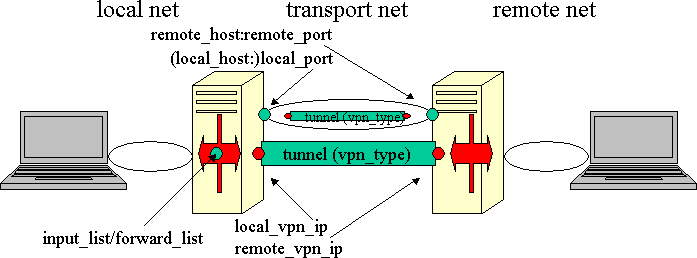
\includegraphics[width=\columnwidth]{openvpn-sample}
    \caption{VPN-Konfigurationsbeispiel --- Tunnel zwischen zwei Routern}
    \label{fig:tunnel}
  \end{figure}

  \begin{description}

  \item [local net, remote net] repräsentieren die beiden Netze, die
  über den Tunnel miteinander verbunden werden sollen. Die beiden zu
  verbindenden Netze müssen in unterschiedlichen TCP/IP Netzen sein
  und dürfen sich in ihren Netzmasken auch nicht überschneiden. Die
  Einstellungen von \jump{IPNETx}{\var{IP\_NET\_x}} in der jeweiligen base.txt
  Konfigurationsdateien dürfen also nicht gleich sein. Es ist also mit
  einem VPN Tunnel nicht möglich zwei Netze miteinander zu verbinden,
  die beide das IP Netz 192.168.6.0/24 benutzen.

  \item [transport net] das Transport Netzwerk besteht aus zwei
  Elementen:

  \begin{itemize}

  \item der Verbindung zwischen zwei OpenVPN-Daemons, beschrieben
  durch \emph{\smalljump{OPENVPNxREMOTEHOST}{remote\_host}:\smalljump{OPENVPNxREMOTEPORT}{remote\_port}}
  und \emph{(\smalljump{OPENVPNxLOCALHOST}{local\_host}:)\smalljump{OPENVPNxLOCALPORT}{local\_port}}. Das
  entspricht den OpenVPN Einstellungen \var{OPENVPN\_x\_REMOTE\_HOST},
  \var{OPENVPN\_x\_REMOTE\_PORT}, \var{OPENVPN\_x\_LOCAL\_HOST} und
  \var{OPENVPN\_x\_LOCAL\_PORT}.

  \item und dem Tunnel, über den die Verbindung zwischen den
  OpenVPN-Daemons etabliert wird, beschrieben durch
  \emph{\smalljump{OPENVPNxLOCALVPNIP}{local\_vpn\_ip}/\smalljump{OPENVPNxREMOTEVPNIP}{remote\_vpn\_ip}}. Dies
  entspricht dann wieder \var{OPENVPN\_x\_LOCAL\_VPN\_IP} und
  \var{OPENVPN\_x\_REMOTE\_VPN\_IP}. Die beiden VPN IP-Adressen dürfen sich
  dabei in keinem anderen, den beiden Routern bekannten Netzen liegen.

  \end{itemize}

  \item [\smalljump{OPENVPNxPFINPUTN}{input\_list},
  \smalljump{OPENVPNxPFFORWARDN}{forward\_list}] Pakete, die über den
  Tunnel gehen sollen, müssen zuerst durch den Paketfilter. Dieser
  erlaubt standardmäßig nur ICMP-Nachrichten (z. B. ping), die man
  zum Testen des Tunnels verwenden kann. Alles andere muß erst
  explizit erlaubt werden, im einfachsten Falle durch

\begin{example}
\begin{verbatim}
OPENVPN_x_PF_INPUT_POLICY='ACCEPT'
OPENVPN_x_PF_FORWARD_POLICY='ACCEPT'
\end{verbatim}
\end{example}

  \achtung{Bitte denken Sie daran, dass das komplette
  \glqq{}Freigeben\grqq{} einer VPN Verbindung sicherheitstechnisch
  sehr bedenklich ist. Benutzen Sie lieber die tmpl: Syntax des
  Paketfilters, um nur gezielt die Dienste freizugeben, die Sie auch
  benötigen.}

  \end{description}

Mehr Einstellungen sind für einen einfachen VPN Tunnel nicht
notwendig. Alle weiteren Einstellmöglichkeiten behandeln erweiterte
Funktionen oder sind für spezielle Anwendungsfälle gedacht. Sie
sollten mit diesen erweiterten Einstellungen erst dann arbeiten, weil
der VPN Tunnel mit den minimalen Einstellungen erfolgreich aufgebaut
werden kann.

\subsection{OpenVPN - Konfiguration}

Da OpenVPN ziemlich komplex ist, beginnen wir mit der Erklärung der
zwingend notwendigen Angaben für jede VPN Verbindung. Erst wenn der
fli4l-Router mit diesen Einstellungen eine Verbindung aufgebaut hat,
sollten Sie sich daran wagen die erweiterten
Konfigurationsmöglichkeiten von OpenVPN zu nutzen.

\begin{description}

\config{OPT\_OPENVPN}{OPT\_OPENVPN}{OPTOPENVPN}

  Default: \var{OPT\_OPENVPN='no'}

  Mit \var{'yes'} wird das OpenVPN Paket aktiviert. Die Einstellung
  \var{'no'} deaktiviert das OpenVPN Paket komplett.

\config{OPENVPN\_N}{OPENVPN\_N}{OPENVPNN}

  Default: \var{OPENVPN\_N='0'}

  Wieviele OpenVPN Konfigurationen sind in der Konfigurationsdatei
  aktiv?

\config{OPENVPN\_x\_REMOTE\_HOST}{OPENVPN\_x\_REMOTE\_HOST}{OPENVPNxREMOTEHOST}

  Default: \var{OPENVPN\_x\_REMOTE\_HOST=''}

  Die IP-Adresse oder eine DNS-Adresse der OpenVPN Gegenstelle. Bei
  einem \jump{roadwarrior}{Roadwarrior} muss diese Zeile komplett
  fehlen.  Wird diese Einstellung weggelassen, wartet OpenVPN auf
  einen Verbindungsaufbau und versucht nicht selbstständig die
  Verbindung aufzubauen.

\config{OPENVPN\_x\_REMOTE\_HOST\_N}{OPENVPN\_x\_REMOTE\_HOST\_N}{OPENVPNxREMOTEHOSTN}

  Default: \var{OPENVPN\_x\_REMOTE\_HOST\_N='0'}

  Bei der Benutzung von dynamischen DNS Diensten passiert es leider ab
  und an, dass ein Dienst nicht 100\% zuverlässig funktioniert. Daher
  macht es in diesen Fällen Sinn, einfach zwei oder mehr DynDNS
  Dienste zu benutzen und seine aktuelle IP-Adresse bei allen Diensten
  gleichzeitig zu registrieren. Damit OpenVPN in diesem Fall auch alle
  DynDNS Namen durchgehen kann, muss hier noch die Liste der
  \emph{zusätzlichen} DNS Namen eingegeben werden. Zusammen mit
  \var{OPENVPN\_x\_REMOTE\_HOST} ergibt sich dann die Liste der DynDNS
  Adressen, die OpenVPN in zufälliger Reihenfolge zu kontaktieren
  versucht. Der Eintrag \var{OPENVPN\_x\_REMOTE\_HOST} muss also
  weiterhin vorhanden sein!

\config{OPENVPN\_x\_REMOTE\_HOST\_x}{OPENVPN\_x\_REMOTE\_HOST\_x}{OPENVPNxREMOTEHOSTx}

  Default: \var{OPENVPN\_x\_REMOTE\_HOST\_x=''}

  Es gilt die gleiche Beschreibung wie unter
  \jump{OPENVPNxREMOTEHOST}{\var{OPENVPN\_x\_REMOTE\_HOST}}.

\config{OPENVPN\_x\_REMOTE\_PORT}{OPENVPN\_x\_REMOTE\_PORT}{OPENVPNxREMOTEPORT}

  Default: \var{OPENVPN\_x\_REMOTE\_PORT=''}

  Jede OpenVPN Verbindung braucht eine auf dem fli4l-Router bisher
  nicht benutzte Portadresse. Es empfiehlt sich, einen Port oberhalb
  von 10000 zu nehmen, da dort normalerweise keine häufig benutzen
  Ports liegen. Wenn Sie eine Verbindung für eine Gegenstelle
  bereitstellen wollen, die eine wechselnde IP-Adresse hat und über
  keine DynDNS Adresse verfügt, lassen Sie diesen Eintrag genau wie
  \var{OPENVPN\_x\_REMOTE\_HOST} komplett weg.

\config{OPENVPN\_x\_LOCAL\_HOST}{OPENVPN\_x\_LOCAL\_HOST}{OPENVPNxLOCALHOST}

  Default: \var{OPENVPN\_x\_LOCAL\_HOST=''}

  Gibt an, an welche IP-Adresse OpenVPN gebunden werden soll. Bei
  Verbindungen über das Internet sollte dieser Eintrag leer bleiben
  oder komplett weggelassen werden.  Wird hier eine IP-Adresse
  angegeben, horcht OpenVPN nur auf dieser IP-Adresse auf eingehende
  Verbindungsanfragen. Wenn Sie eine WLAN Verbindung absichern wollen,
  sollten Sie hier die IP-Adresse der WLAN Karte vom fli4l-Router
  eintragen.

\config{OPENVPN\_x\_LOCAL\_PORT}{OPENVPN\_x\_LOCAL\_PORT}{OPENVPNxLOCALPORT}

  Default: \var{OPENVPN\_x\_LOCAL\_PORT=''}

  Gibt die Portnummer an, auf der der lokale OpenVPN Daemon
  horcht. Für jede OpenVPN Einstellung benötigen Sie einen dafür
  reservierten Port, d.h. dieser Port kann nur von dieser einer
  OpenVPN Verbindung benutzt werden und darf auch von keiner anderen
  Software auf dem fli4l-Router benutzt werden.  Die Einstellungen
  \var{OPENVPN\_x\_REMOTE\_PORT} und \var{OPENVPN\_x\_LOCAL\_PORT}
  jeder OpenVPN Verbindung müssen zusammenpassen! Wenn Sie auf einer
  Seite des Tunnel \var{OPENVPN\_x\_REMOTE\_PORT='10111'} setzen
  \emph{muss} die andere zwingend auf
  \var{OPENVPN\_x\_LOCAL\_PORT='10111'} gesetzt werden.

  Nochmal: Es ist sehr wichtig, diese Einstellungen auf die jeweilige
  OpenVPN Gegenstelle anzupassen, sonst ist eine Verbindung zwischen
  den OpenVPN Partnern nicht möglich.

  Damit OpenVPN auf eingehende Verbindungen horchen kann, öffnet
  OpenVPN selbstständig die Ports im Paketfilter, die unter
  \var{OPENVPN\_x\_LOCAL\_PORT} angegeben werden. Wenn dies nicht
  gewünscht wird, können Sie dies unter
  \jump{OPENVPNDEFAULTOPENOVPNPORT}{\var{OPENVPN\_DEFAULT\_OPEN\_OVPNPORT}}
  anpassen. Es ist \emph{nicht} notwendig den Eintrag
  \var{OPENVPN\_DEFAULT\_OPEN\_OVPNPORT='yes'} zu setzen, da das die
  Standardeinstellung ist!

  Es ist nicht möglich OpenVPN auf Ports kleiner als 1025 horchen zu
  lassen. Wenn Sie z.B. einen OpenVPN als tcp4- oder tcp6-server auf Port 443
  (der https Port) konfigurieren wollen, müssen Sie den Port 443 per
  Paketfilter an einen Port über 1024 weiterleiten. Wenn Sie z.B. den
  OpenVPN auf Port 5555 horchen lassen und den Port 443 weiterleiten
  wollen, muss folgendes in die \var{PF\_PREROUTING} eingetragen werden.

\begin{example}
\begin{verbatim}
PF_PREROUTING_5='tmpl:https dynamic REDIRECT:5555'
\end{verbatim}
\end{example}

\config{OPENVPN\_x\_SECRET}{OPENVPN\_x\_SECRET}{OPENVPNxSECRET}

  Default: \var{OPENVPN\_x\_SECRET=''}

  OpenVPN benötigt zum Verschlüsseln der OpenVPN Verbindung ein
  sogenanntes Keyfile. Dieses Keyfile kann unter Windows oder Linux
  direkt mit OpenVPN erzeugt werden. Für Anfänger bietet es sich an,
  die Windows Software von OpenVPN zu installieren oder die OpenVPN
  WebGUI zu benutzen. Wenn Sie OpenVPN unter Windows nicht einsetzen
  wollen, sondern nur die für OpenVPN benötigen Keyfiles erstellen
  wollen, reicht es, die Punkte \emph{OpenVPN User-Space Components},
  \emph{OpenSSL DDLs}, \emph{OpenSSL Utilities}, \emph{Add OpenVPN to
  PATH} und \emph{Add Shortcuts to OpenVPN} zu installieren. Mit dem
  Menüpunkt \emph{Generate a static OpenVPN key}, den Sie im Startmenü
  unter OpenVPN finden, können dann die benötigten Keydateien erzeugt
  werden. Nach dem Aufruf des Menüpunktes kommt die Meldung
  \glqq{}Randomly generated 2048 bit key written to
  \var{C:/Programme/OpenVPN/config/key.txt}\grqq{}. Die erstellte
  \var{key.txt} Datei ist das benötigte Keyfile. Kopieren Sie diese
  Datei einfach in das Verzeichnis \var{$<$config$>$/etc/openvpn} und
  bennenen Sie die \var{key.txt} entsprechend um, so dass der
  Dateiname aussagekräftig wird. Sie können ein Keyfile auch
  automatisch vom fli4l-Router erstellen lassen, wenn Sie
  \var{OPENVPN\_CREATE\_SECRET} auf \var{'yes'} stellen und den
  fli4l-Router neu starten. Wenn Sie also das erste Mal OpenVPN
  konfigurieren, tragen Sie alle Daten in die Konfigdatei ein und
  setzen entweder
  \jump{OPENVPNDEFAULTCREATESECRET}{\var{OPENVPN\_DEFAULT\_CREATE\_SECRET}}
  auf \var{'yes'}, wenn Sie gleich für alle OpenVPN Verbindungen neue
  Keyfiles erzeugen wollen oder nur für die entsprechende OpenVPN
  Verbindung \var{OPENVPN\_x\_CREATE\_SECRET} auf \var{'yes'}. Nach
  dem Start des fli4l-Routers werden dann die oder das Keyfile(s)
  automatisch erzeugt und in \var{/etc/openvpn} mit dem hier
  angegebenen Namen abgelegt.  Das oder die Keyfile(s) kann dann per
  scp kopiert oder mit einer Diskette übertragen werden.  Sie müssen
  nach dem Erstellen der Schlüsseldateien die Einstellung wieder auf
  'no' setzen, das fli4l Bootmedium neu erzeugen und die neu
  erzeugte Konfiguration starten. Bleibt die Einstellung auf 'yes'
  werden bei jedem Start des fli4l-Routers neue Schlüsseldateien
  erzeugt aber kein OpenVPN Daemon gestartet. Es also kann kein Tunnel
  aufgebaut werden. Sie können \var{OPENVPN\_x\_CREATE\_SECRET} auch
  auf \var{'webgui'} setzen, wenn Sie die WebGUI verwenden möchten um
  Keyfile(s) zu generieren. Dazu müssen Sie in der WebGUI in die
  Detailansicht der Verbindung(en) gehen und den Punkt Keymanagement
  auswählen. Genaueres dazu im Abschnitt \ref{sec:openvpn_gui}

  Tipp: Mit dem Kommando 
  \begin{verbatim}
      openvpn --genkey --secret <dateiname>
  \end{verbatim}
  können Sie ein Keyfile auf dem fli4l-Router auch von Hand erstellen.

  Die Keyfiles müssen in das Verzeichnis
  \var{$<$config$>$/etc/openvpn} kopiert werden, wie in folgendem Bild
  zu sehen ist. Der Dateiname des Keyfiles ohne den Pfad muss
  anschließend in \var{OPENVPN\_x\_SECRET} hinterlegt werden. Dann
  werden die Keyfiles beim Erstellen des opt-Archives mit eingepackt.

  \begin{figure}[htbp]
    \centering
    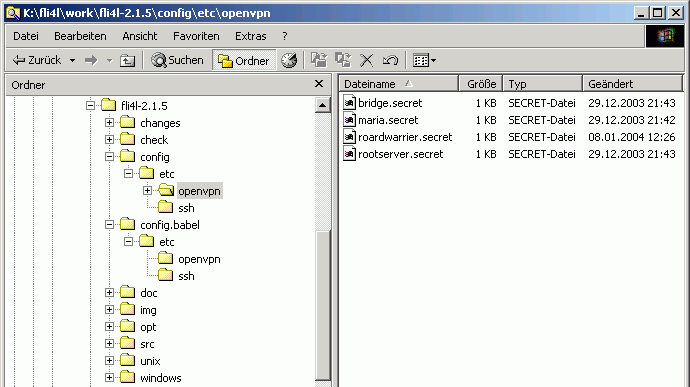
\includegraphics[width=\columnwidth]{config_etc_openvpn}
    \caption{fli4l config Directory mit OpenVPN *.secret Dateien}
    \label{fig:config_etc_openvpn}
  \end{figure}

\config{OPENVPN\_x\_TYPE}{OPENVPN\_x\_TYPE}{OPENVPNxTYPE}

  Default: \var{OPENVPN\_x\_TYPE=''}

  Eine OpenVPN Verbindung kann entweder als Tunnel oder als Bridge
  benutzt werden. Über einen OpenVPN Tunnel kann ausschliesslich
  IP-Traffic geroutet werden. Über eine Bridge werden Ethernetframes
  übertragen, also nicht nur IP-Traffic, sondern z.B. auch IPX oder
  NetBEUI. Wenn OpenVPN als Transport für Ethernetframes benutzt werden
  soll, wird in jedem Fall noch das advanced\_networking Paket
  benötigt. Bitte bedenken Sie, dass die Benutzung von Bridging über
  eine DSL Leitung sehr langsam werden kann!

\end{description}

\subsection{OpenVPN - Bridgekonfiguration}

  Wenn Sie OpenVPN für eine Bridge benutzen wollen, sind folgende
  Einträge gültig. Bitte denken Sie daran, dass bei der Benutzung
  einer Bridge über das Internet der entstehende Broadcasttraffic
  unter Umständen schon eine relativ hohe Bandbreite benötigt.

  Denken Sie daran, dass die folgenden Einstellungen nur gültig sind,
  wenn der \jump{OPENVPNxTYPE}{\var{OPENVPN\_x\_TYPE}} für diese OpenVPN
  Verbindung auf \var{'bridge'} eingestellt wurde! Ausserdem wird eine
  konfigurierte Bridge aus dem advanced\_networking Paket benötigt, an
  die sich die VPN Verbindung hängen kann.

\begin{description}

\config{OPENVPN\_x\_BRIDGE}{OPENVPN\_x\_BRIDGE}{OPENVPNxBRIDGE}

  Default: \var{OPENVPN\_x\_BRIDGE=''}

  Hier wird der Name der Bridge angegeben, an die sich diese OpenVPN
  Verbindung hängen soll.  Wenn also in
  \var{BRIDGE\_DEV\_x\_NAME='cuj-br'} steht und sich diese OpenVPN
  Verbindung an diese Bridge hängen soll, muss hier ebenfalls
  \var{'cuj-br'} angegeben werden.

\config{OPENVPN\_x\_BRIDGE\_COST}{OPENVPN\_x\_BRIDGE\_COST}{OPENVPNxBRIDGECOST}

  Default: \var{OPENVPN\_x\_BRIDGE\_COST=''}

  Wenn Sie STP (siehe
  \altlink{http://de.wikipedia.org/wiki/Spanning_Tree} oder die
  Dokumentation im advanced\_networking Paket) benutzen, können Sie
  hier die Kosten der Verbindung angeben.

\config{OPENVPN\_x\_BRIDGE\_PRIORITY}{OPENVPN\_x\_BRIDGE\_PRIORITY}{OPENVPNxBRIDGEPRIORITY}

  Default: \var{OPENVPN\_x\_BRIDGE\_PRIORITY=''}

  Wenn Sie STP (siehe
  \altlink{http://de.wikipedia.org/wiki/Spanning_Tree} oder die
  Dokumentation im advanced\_networking Paket) benutzen, können Sie
  hier die Priorität der Verbindung angeben.

\end{description}

\subsection{OpenVPN - Tunnelkonfiguration}

\begin{description}

\config{OPENVPN\_x\_REMOTE\_VPN\_IP}{OPENVPN\_x\_REMOTE\_VPN\_IP}{OPENVPNxREMOTEVPNIP}

  Default: \var{OPENVPN\_x\_REMOTE\_VPN\_IP=''}

  Diese Einstellung ist nur gültig, wenn der
  \jump{OPENVPNxTYPE}{\var{OPENVPN\_x\_TYPE}} für diese OpenVPN Verbindung
  auf \var{'tunnel'} einstellt wurde!

  Die VPN IP-Adresse der OpenVPN Gegenstelle. Die VPN IP-Adressen
  werden nur zum Routen benötigt und können fast frei gewählt
  werden. Es gelten dabei folgende Einschränkungen für die Auswahl der
  VPN IP-Adressen:

\begin{itemize}

\item Die IP-Adresse darf an keiner Stelle im lokalen Netz benutzt werden. Sie darf also nicht im Subnetz des fli4l-Routers liegen.

\item Die IP-Adresse darf für kein lokales Netzwerkdevice benutzt werden.

\item Die IP-Adresse darf nicht zu einem Netzwerk gehören, das mit \var{IP\_ROUTE\_x} geroutet wird.

\item Die IP-Adresse darf nicht zu einem Netzwerk gehören, das mit \var{ISDN\_CIRC\_ROUTE\_x} geroutet wird.

\item Die IP-Adresse darf nicht zu einem Netzwerk gehören, das mit \var{CIPE\_ROUTE\_x} geroutet wird.

\item Die IP-Adresse darf nicht zu einem Netzwerk gehören, das mit \var{OPENVPN\_ROUTE\_x} geroutet wird.

\item Die IP-Adresse darf nicht zu einem Netzwerk gehören, das auf irgendeine andere Weise zum fli4l Netzwerk gehört oder vom fli4l-Router geroutet wird.

\end{itemize}

  Wie Sie sehen darf die VPN IP-Adresse nirgends sonst benutzt
  werden. Bevor Sie mit der Konfiguration von OpenVPN beginnen,
  sollten Sie sich ein Netz suchen, was von keinem Netzwerk benutzt
  wird, in das Sie eine VPN Verbindung aufbauen wollen. Das Netzwerk
  sollte auch unbedingt zu einem der privaten Netze gehören (siehe
  \altlink{http://ftp.univie.ac.at/netinfo/rfc/rfc1597.txt}).

\config{OPENVPN\_x\_LOCAL\_VPN\_IP}{OPENVPN\_x\_LOCAL\_VPN\_IP}{OPENVPNxLOCALVPNIP}

  Default: \var{OPENVPN\_x\_LOCAL\_VPN\_IP=''}

  Diese Einstellung ist nur gültig, wenn der
  \jump{OPENVPNxTYPE}{\var{OPENVPN\_x\_TYPE}} für diese OpenVPN Verbindung
  auf \var{'tunnel'} einstellt wurde.

  Die IP-Adresse, die das lokale OpenVPN tunX Device bekommt. Für die
  Auswahl der IP-Adresse gelten die gleichen Einschränkungen wie bei
  \jump{OPENVPNxREMOTEVPNIP}{\var{OPENVPN\_x\_REMOTE\_VPN\_IP}}.

  Es ist übrigens möglich, für alle lokalen OpenVPN Verbindungen die
  gleiche IP-Adresse bei \var{OPENVPN\_x\_LOCAL\_VPN\_IP} zu
  benutzen. So ist es problemlos möglich, dass ein Host in einem VPN
  immer die gleiche IP-Adresse benutzt. Das vereinfacht die
  Paketfilterregeln unter Umständen drastisch.
  
\config{OPENVPN\_x\_IPV6}{OPENVPN\_x\_IPV6}{OPENVPNIPV6}

  Default: \var{OPENVPN\_x\_IPV6='no'}
  
  Hiermit kann der native IPv6-Support von OpenVPN eingeschaltet werden. Da dieser Code 
  noch recht neu ist, ist der Support als experimentell zu bezeichnen. Damit das Ganze einen 
  Effekt hat, muss OPT\_IPV6 aktiviert und konfiguriert sein. Bei \var{OPENVPN\_x\_IPV6='no'}
  und/oder \var{OPT\_IPV6='no'} werden die IPv6 relevanten Variablen ignoriert. 
  
  ACHTUNG!!! Zur Zeit gibt es hier keine Überprüfung ob sich die Angaben mit anderen Teilen 
  der Konfiguration überschneiden! Dies gilt für \var{OPENVPN\_x\_LOCAL\_VPN\_IPV6},
  \var{OPENVPN\_x\_REMOTE\_VPN\_IPV6} und \var{OPENVPN\_x\_ROUTE\_x}.
  
\config{OPENVPN\_x\_REMOTE\_VPN\_IPV6}{OPENVPN\_x\_REMOTE\_VPN\_IPV6}{OPENVPNxREMOTEVPNIPV6}

  Default: \var{OPENVPN\_x\_REMOTE\_VPN\_IPV6=''}
  
  Für die IPv6 gilt das Gleiche wie für die \jump{OPENVPNxREMOTEVPNIP}{\var{OPENVPN\_x\_REMOTE\_VPN\_IP}}.
  
  \begin{example}
  \begin{verbatim}
    OPENVPN_X_REMOTE_IPV6='FD00::1'
  \end{verbatim}
  \end{example}

\config{OPENVPN\_x\_LOCAL\_VPN\_IPV6}{OPENVPN\_x\_LOCAL\_VPN\_IPV6}{OPENVPNxLOCALVPNIPV6}

  Default: \var{OPENVPN\_x\_LOCAL\_VPN\_IPV6=''}
  
  Für die IPv6 gilt das Gleiche wie für die \jump{OPENVPNxLOCALVPNIP}{\var{OPENVPN\_x\_LOCAL\_VPN\_IP}}.
  Wird hier kein Subnetz gesetzt wird automatisch /64 als Subnetz genutzt.
  
  \begin{example}
  \begin{verbatim}
    OPENVPN_X_LOCAL_IPV6='FD00::2/112'
  \end{verbatim}
  \end{example}

\config{OPENVPN\_x\_ROUTE\_N}{OPENVPN\_x\_ROUTE\_N}{OPENVPNxROUTEN}

  Default: \var{OPENVPN\_x\_ROUTE\_N=''}

  Diese Einstellung ist nur gültig, wenn der
  \jump{OPENVPNxTYPE}{\var{OPENVPN\_x\_TYPE}} für diese OpenVPN Verbindung
  auf \var{'tunnel'} einstellt wurde.

  Die angegebenen Routen werden automatisch von OpenVPN gesetzt,
  sobald OpenVPN gestartet wird. Es können bis zu 50 Netze über eine
  OpenVPN Verbindung geroutet werden. Sie müssen aber für jedes zu
  routende Netzwerk einen \var{OPENVPN\_x\_ROUTE\_x} Eintrag erzeugen.

  Bitte beachten Sie, dass Sie notwendige Paketfilterregeln in der
  \var{OPENVPN\_PF\_FORWARD\_x} \var{OPENVPN\_PF\_INPUT\_x} bzw
  \var{OPENVPN\_PF6\_FORWARD\_x} \var{OPENVPN\_PF6\_INPUT\_x} bzw
  selber setzen müssen. OpenVPN erlaubt nur ICMP über die VPN
  Verbindungen und verbietet allen anderen Datenverkehr. Details
  finden Sie unter
  \jump{OPENVPNxPFINPUTN}{\var{OPENVPN\_x\_PF\_INPUT\_N}} und
  \jump{OPENVPNxPFFORWARDN}{\var{OPENVPN\_x\_PF\_FORWARD\_N}} bzw.
  unter
  \jump{OPENVPNxPF6INPUTN}{\var{OPENVPN\_x\_PF6\_INPUT\_N}} und
  \jump{OPENVPNxPF6FORWARDN}{\var{OPENVPN\_x\_PF6\_FORWARD\_N}} bzw.
  
  Für sehr spezielle Konfigurationen besteht die Möglichkeit, Skripte
  zu starten um z.B. Policy Based Routing zu ermöglichen. Die Skripte
  müssen dazu in dem Verzeichnis \texttt{config/etc/openvpn} abgelegt
  werden und folgendermaßen benannt werden:

\begin{example}
  <name>-<zeitpunkt>
\end{example}

  Der ``name'' ist der Name der OpenVPN-Verbindung
  (\var{OPENVPN\_x\_NAME}).  Für ``zeitpunkt'' stehen folgende
  Auswahlmöglichkeiten für die Ausführung der Skripte zur Verfügung:

  \begin{itemize}
    \item [up-pre] Vor dem Herstellen der OpenVPN-Verbindung.
    \item [up-post] Nach dem Herstellen der OpenVPN-Verbindung.
    \item [down-pre] Vor dem Abbau der OpenVPN-Verbindung.
    \item [down-post] Nach dem Abbau der OpenVPN-Verbindung.
    \item [route-up-pre] Vor dem Setzen der OpenVPN-Routen.
    \item [route-up-post] Nach dem Setzen der OpenVPN-Routen.
    \item [route-down-pre] Vor dem Löschen der OpenVPN-Routen.
    \item [route-down-post] Nach dem Löschen der OpenVPN-Routen.
  \end{itemize}

  Um ein Skript für die Verbindung \var{OPENVPN\_x\_NAME='maria'} nach
  dem Setzen der Routen zu starten muss ein Skript mit dem
  Namen \texttt{maria-route-up-post} in dem
  Verzeichnis \texttt{config/etc/openvpn} angelegt werden.

\config{OPENVPN\_x\_ROUTE\_x}{OPENVPN\_x\_ROUTE\_x}{OPENVPNxROUTEx}

  Default: \var{OPENVPN\_x\_ROUTE\_x=''}

  Sie müssen hier die Netze angeben, die Sie über die OpenVPN
  Gegenstelle erreichen wollen. Sind hinter der OpenVPN Gegenstelle
  z.B. die Netzwerke 192.168.33.0/24 und 172.18.0.0/16 erreichbar und
  sollen diese über den OpenVPN Tunnel erreicht werden, müssen Sie
  diese beiden Netze jeweils einzeln unter \var{OPENVPN\_x\_ROUTE\_x}
  eintragen. Es können hier auch Hostrouten (\var{/32}) eingetragen
  werden.

  Wenn die Defaultroute über einen OpenVPN Tunnel gesetzt werden soll,
  geben sie bitte 0.0.0.0/0 bzw. ::/0 für IPv6 und ein 
  optionales Flag als Route an. Auch hier gilt, das für IPv6 Routen OPT\_IPv6 
  aktiv sein muss, die lokale und remote IPv6-Adresse für den Tunnel müssen gesetzt 
  sein und OPENVPN\_x\_IPV6 auf yes stehen. OpenVPN kennt verschiedene Möglichkeiten 
  die Defaultroute einzurichten, die sie mit dem Flag auswählen können. 
  Jede Methode, die Defaultroute einzurichten, hat ihre Vor- und Nachteile. 
  Im Moment unterstützt OpenVPN folgende Flags:

\begin{itemize}
\item [local] Das \emph{local} Flag sollten sie wählen, wenn die
              OpenVPN Gegenstelle innerhalb eines direkt von ihrem
              fli4l-Router erreichbaren Subnetz liegt. Das ist
              z.B. oft bei einer Defaultroute mit OpenVPN über WLAN
              der Fall.
\item [def1] Mit diesem Flag werden zusätzliche zu einer Hostroute an
             die OpenVPN Gegenstelle zwei neue Routen, 0.0.0.0/1 und
             128.0.0.0/1, eingetragen. Diese Routen übernehmen die
             Funktion einer Defaultroute und über diese Routen wird
             dann der komplette (verschlüsselte) Traffic an die
             OpenVPN Gegenstelle (die noch über die Hostroute
             erreichbar ist) geroutet.
\end{itemize}

  Lassen Sie das optionale Flag weg wählt OpenVPN die Methode aus, wie
  die Defaultroute umgesetzt wird. Die Auswahl der Methode erfolgt
  dabei über die OpenVPN Version, im Moment wird als
  Standardeinstellung \emph{local} benutzt.

\begin{example}
\begin{verbatim}
OPENVPN_1_ROUTE_N='3'
OPENVPN_1_ROUTE_1='192.168.33.0/24'
OPENVPN_1_ROUTE_2='172.18.0.0/16'
OPENVPN_1_ROUTE_3='2001:db8:/32'
\end{verbatim}
\end{example}

\end{description}

\subsubsection{OpenVPN - Delegation von DNS und Reverse-DNS}

\begin{description}

\config{OPENVPN\_x\_DOMAIN}{OPENVPN\_x\_DOMAIN}{OPENVPNxDOMAIN}

  Default: \var{OPENVPN\_x\_DOMAIN=''}

  Über diesen Parameter gibt man die Remote Domain an. Diese Variable kann
  mehrere Domains enthalten die durch Leerzeichen getrennt angegeben werden
  müssen. Wenn nur dieser Parameter gesetzt ist (ohne Angabe eines
  zusätzlichen DNS-Servers) wird davon ausgegangen, dass der DNS Server auf der
  IP des gegenüberliegenden Tunnelendes lauscht (siehe \jump{OPENVPNxREMOTEVPNIP}{\var{OPENVPN\_x\_REMOTE\_VPN\_IP}}).
  Dazu müssen auf dem Remote Router natürlich eingehende DNS-Anfragen erlaubt werden.
  (z.B. via \var{OPENVPN\_x\_INPUT\_y='tmpl:dns ACCEPT'})

\config{OPENVPN\_x\_ROUTE\_x\_DOMAIN}{OPENVPN\_x\_ROUTE\_x\_DOMAIN}{OPENVPNxROUTExDOMAIN}

  Default: \var{OPENVPN\_x\_ROUTE\_x\_DOMAIN=''}

  Den verschiedenen Subnetzen können auch verschiedene Domains zugeordnet sein.
  Hier kann man pro \var{OPENVPN\_x\_ROUTE\_y} eine entsprechende Domain konfigurieren.
  Sollte ein dazugehöriges \var{OPENVPN\_x\_ROUTE\_y\_DNSIP} existieren, so wird dieser Server
  benutzt, andernfalls der unter \var{OPENVPN\_x\_DNSIP} angegebene. Die Wirkung ist
  dann die selbe wie mit \var{OPENVPN\_x\_DOMAIN}, allerdings eignet sich diese Methode
  auch zur Dokumentation.

\config{OPENVPN\_x\_DNSIP}{OPENVPN\_x\_DNSIP}{OPENVPNxDNSIP}

  Default: \var{OPENVPN\_x\_DNSIP=''}

  Ist der Tunnelendpunkt nicht der zuständige DNS-Server, so kann hier die IP
  des zuständigen DNS-Servers angegeben werden.
  Ist nichts angegeben, wird die unter \jump{OPENVPNxREMOTEVPNIP}{\var{OPENVPN\_x\_REMOTE\_VPN\_IP}} angegebene IP
  benutzt.

\config{OPENVPN\_x\_ROUTE\_x\_DNSIP}{OPENVPN\_x\_ROUTE\_x\_DNSIP}{OPENVPNxROUTExDNSIP}

  Default: \var{OPENVPN\_x\_ROUTE\_x\_DNSIP=''}

  Verschiedene geroutete Subnetze können auch durch verschiedene DNS-Server
  abgedeckt sein - hier kann man pro \jump{OPENVPNxROUTEx}{\var{OPENVPN\_x\_ROUTE\_x}} einen eigenen
  zuständigen Server definieren.

\end{description}

\subsection{Experteneinstellungen}

Die in diesem Kapitel beschriebenen Einstellungen sind fast alle optional
und sollten nur verändert werden, wenn die OpenVPN Verbindung mit den
Standardeinstellungen funktioniert und Optimierungen (beispielsweise eine
andere Schlüssellänge) vorgenommen werden sollen.

Mit Ausnahme von \var{OPENVPN\_DEFAULT\_CIPHER} und
\var{OPENVPN\_DEFAULT\_DIGEST} sind alle nachfolgend beschriebenen
\var{OPENVPN\_DEFAULT\_} Einstellungen optional, d.h. diese Optionen brauchen
nicht in die \texttt{openvpn.txt} Konfigurationsdatei geschrieben werden. Fehlt
der entsprechende Eintrag in der openvpn.txt Datei, wird vom OpenVPN Startskript
der hier angegebene Defaultwert benutzt. Wenn Sie nicht vorhaben die
Standardwerte der Vorgaben zu änden, schreiben Sie diese auch nicht in
die openvpn.txt Konfigurationsdatei!

\subsubsection{allgemeine Einstellungen}

\begin{description}

\config{OPENVPN\_DEFAULT\_CIPHER}{OPENVPN\_DEFAULT\_CIPHER}{OPENVPNDEFAULTCIPHER}

  Hier wird eine der verfügbaren Verschlüsselungsmethoden eingetragen. Zur Zeit
  werden die Verschlüsselungsmethoden in Tab.~\ref{openvpn:ciphers} unterstützt.

  \begin{table}[!ht]
    \centering
    \caption{In OpenVPN verfügbare Verschlüsselungsmethoden}
    \label{openvpn:ciphers}
    \begin{tabular}{|p{4cm}|r|r|l|}
      \hline
      Kürzel           & nominale Schlüssellänge & effektive Schlüssellänge & Bewertung \\
      \hline
      none             &   0 Bit &   0 Bit & unsicher \\
      DES-CBC          &  56 Bit &  56 Bit & unsicher \\
      DES-EDE-CBC      & 112 Bit &  80 Bit & unsicher \\
      DES-EDE3-CBC     & 168 Bit & 112 Bit & unsicher \\
      DESX-CBC         & 184 Bit & 119 Bit & unsicher \\
      RC2-40-CBC       &  40 Bit &  40 Bit & unsicher \\
      RC2-64-CBC       &  64 Bit &  64 Bit & unsicher \\
      RC2-CBC          & 128 Bit & 128 Bit & unsicher \\
      BF-CBC           & 128 Bit & 128 Bit & sicher \\
      CAST5-CBC        & 128 Bit & 128 Bit & sicher \\
      AES-128-CBC      & 128 Bit & 128 Bit & sicher \\
      AES-192-CBC      & 192 Bit & 192 Bit & sicher \\
      AES-256-CBC      & 256 Bit & 256 Bit & sicher \\
      CAMELLIA-128-CBC & 128 Bit & 128 Bit & sicher \\
      CAMELLIA-192-CBC & 192 Bit & 192 Bit & sicher \\
      CAMELLIA-256-CBC & 256 Bit & 256 Bit & sicher \\
      SEED-CBC         & 128 Bit & 128 Bit & sicher \\
      \hline
    \end{tabular}
  \end{table}

  \wichtig{Diese Variable hat \emph{keine} Vorbelegung! Sie müssen somit einen
  Algorithmus auswählen. Falls Sie unsicher sind, wählen Sie
  \begin{itemize}
  \item ``AES-128-CBC'', wenn Sie dafür Hardware-Unterstützung nutzen können
        (siehe Paket ``hwsupp''), oder
  \item ``AES-256-CBC'', wenn Sie eine schnelle CPU haben (1 GHz oder
        schneller), oder
  \item ``BF-CBC'' in allen anderen Fällen.
  \end{itemize}}

  In alten Versionen von fli4l war diese Variable in der Standardeinstellung mit
  ``BF-CBC'' belegt.

\config{OPENVPN\_DEFAULT\_COMPRESS}{OPENVPN\_DEFAULT\_COMPRESS}{OPENVPNDEFAULTCOMPRESS}

  Default: \var{OPENVPN\_DEFAULT\_COMPRESS='yes'}

  OpenVPN benutzt eine adaptive LZO Datenkomprimierung, um die
  Bandbreite einer Verbindung zu erhöhen. Adaptiv bedeutet, dass
  OpenVPN selbstständig erkennt, wenn z.B. bereits gepackte ZIP
  Dateien über eine OpenVPN Verbindung geschickt werden. In einem
  solchen Fall wird die Datenkomprimierung solange abgeschaltet, bis
  wieder Daten übertragen werden, die auch von einer
  Datenkomprimierung profitieren.  Es gibt fast nie einen Grund die
  Datenkomprimierung zu deaktiveren, da dadurch die Bandbreite quasi
  kostenlos erhöht wird. Einziger Nachteil der Datenkomprimierung ist
  eine geringe Erhöhung der Latenzzeit von wenigen Millisekunden. Für
  Online-Games via VPN, bei denen die Reaktionszeit (''guter'' ping)
  entscheidend ist, wäre es also unter Umständen sinnvoll die
  Datenkomprimierung abzuschalten.

\config{OPENVPN\_DEFAULT\_CREATE\_SECRET}{OPENVPN\_DEFAULT\_CREATE\_SECRET}{OPENVPNDEFAULTCREATESECRET}

  Default: \var{OPENVPN\_DEFAULT\_CREATE\_SECRET='no'}

  Mit dieser Einstellung erstellt OpenVPN automatisch Keyfiles beim
  Start des fli4l-Routers. Die entsprechende OpenVPN Verbindung wird
  allerdings nicht gestartet. Für Details lesen Sie bitte den Punkt
  \jump{OPENVPNxSECRET}{\var{OPENVPN\_x\_SECRET}} nach.

\config{OPENVPN\_DEFAULT\_DIGEST}{OPENVPN\_DEFAULT\_DIGEST}{OPENVPNDEFAULTDIGEST}

  Hier wird eine der verfügbaren Prüfsummenmethoden eingetragen. Zur Zeit
  werden die Prüfsummenmethoden in Tab.~\ref{openvpn:digests} unterstützt.

  \begin{table}[!ht]
    \centering
    \caption{In OpenVPN verfügbare Prüfsummenmethoden}
    \label{openvpn:digests}
    \begin{tabular}{|p{4cm}|r|l|}
      \hline
      Kürzel           & Prüfsummenlänge & Bewertung \\
      \hline
      none             &   0 Bit & unsicher \\
      MD4              & 128 Bit & unsicher \\
      RSA-MD4          & 128 Bit & unsicher \\
      MD5              & 128 Bit & unsicher \\
      RSA-MD5          & 128 Bit & unsicher \\
      MDC2             & 128 Bit & sicher \\
      RSA-MDC2         & 128 Bit & sicher \\
      SHA              & 160 Bit & unsicher \\
      RSA-SHA          & 160 Bit & unsicher \\
      SHA1             & 160 Bit & unsicher \\
      RSA-SHA1         & 160 Bit & unsicher \\
      DSA-SHA          & 160 Bit & unsicher \\
      DSA-SHA1-old     & 160 Bit & unsicher \\
      DSA-SHA1         & 160 Bit & unsicher \\
      RSA-SHA1-2       & 160 Bit & unsicher \\
      DSA              & 160 Bit & unsicher \\
      RIPEMD160        & 160 Bit & sicher \\
      RSA-RIPEMD160    & 160 Bit & sicher \\
      ecdsa-with-SHA1  & 160 Bit & sicher \\
      SHA224           & 224 Bit & sicher \\
      RSA-SHA224       & 224 Bit & sicher \\
      SHA256           & 256 Bit & sicher \\
      RSA-SHA256       & 256 Bit & sicher \\
      SHA384           & 384 Bit & sicher \\
      RSA-SHA384       & 384 Bit & sicher \\
      SHA512           & 512 Bit & sicher \\
      RSA-SHA512       & 512 Bit & sicher \\
      whirlpool        & 512 Bit & sicher \\
      \hline
    \end{tabular}
  \end{table}

  \wichtig{Diese Variable hat \emph{keine} Vorbelegung! Sie müssen somit einen
  Algorithmus auswählen. Falls Sie unsicher sind, wählen Sie
  \begin{itemize}
  \item ``whirlpool'', wenn Sie eine schnelle CPU haben (1 GHz oder schneller),
        oder
  \item ``SHA256'' sonst.
  \end{itemize}}

  In alten Versionen von fli4l war diese Variable in der Standardeinstellung mit
  ``SHA1'' belegt.

\config{OPENVPN\_DEFAULT\_FLOAT}{OPENVPN\_DEFAULT\_FLOAT}{OPENVPNDEFAULTFLOAT}

  Default: \var{OPENVPN\_DEFAULT\_FLOAT='yes'}

  Bei OpenVPN Verbindungen mit Gegenstellen, die eine DynDNS Adresse
  benutzen, ist es jederzeit möglich, dass sich die IP-Adresse der
  OpenVPN Gegenstelle ändert. Damit OpenVPN auch die geänderte
  IP-Adresse akzeptiert, muss \var{OPENVPN\_DEFAULT\_FLOAT} auf
  \var{'yes'} eingestellt werden. Mit der Einstellung \var{'no'} wird
  die Änderung der IP-Adresse nicht erlaubt. Das ist in der Regel nur
  bei WLAN Verbindungen oder OpenVPN Verbindungen mit Gegenstellen,
  die eine statische IP-Adresse (wie z.B. die rootserver diverser
  Anbieter) haben, sinnvoll. Sie können diese Einstellung auch wie
  alle anderen \var{OPENVPN\_DEFAULT\_} Einstellungen für eine
  bestimmte OpenVPN Verbindung überschreiben.

\config{OPENVPN\_DEFAULT\_KEYSIZE}{OPENVPN\_DEFAULT\_KEYSIZE}{OPENVPNDEFAULTKEYSIZE}

  Default: \var{OPENVPN\_DEFAULT\_KEYSIZE=''}

  Die Schlüssellänge (=KEYSIZE) hängt von der verwendeten
  Verschlüsselungsmethode ab. Ändern Sie diese Einstellung nur, wenn
  Sie mit einer OpenVPN Gegenstelle zusammenarbeiten müssen, die nicht
  den Standardwert benutzt oder deren Einstellung Sie nicht
  beeinflussen können. Können Sie die Schlüssellänge selbst bestimmen,
  sollte dieser Wert immer leer bleiben. OpenVPN wendet dann eine
  optimale Schlüssellänge für die jeweilige Verschlüsselungmethode an.

\config{OPENVPN\_DEFAULT\_OPEN\_OVPNPORT}{OPENVPN\_DEFAULT\_OPEN\_OVPNPORT}{OPENVPNDEFAULTOPENOVPNPORT}

  Default: \var{OPENVPN\_DEFAULT\_OPEN\_OVPNPORT='yes'}

  Damit eine OpenVPN Gegenstelle mit Ihnen Kontakt aufnehmen kann,
  müssen Sie den Paketfilter Ihres fli4l-Routers entsprechend
  anpassen. In der Regel müssen Sie also auf allen TCP oder UDP Ports,
  je nach \var{OPENVPN\_x\_PROTOCOL} Einstellung, auf denen ein
  OpenVPN horcht, die \jump{PFNEWCONFIG}{\var{PF\_INPUT\_x}} in der
  base.txt anpassen. Mit der Einstellung \var{'yes'} werden diese
  Paketfilterregeln automatisch generiert. Bei einzelnen Verbindungen
  kann es aber durchaus Sinn machen, diese Einstellung auf \var{'no'}
  zu setzen und selber entsprechende Paketfilterregeln zu definieren.

\config{OPENVPN\_DEFAULT\_ALLOW\_ICMPPING}{OPENVPN\_DEFAULT\_ALLOW\_ICMPPING}{OPENVPNDEFAULTALLOWICMPPING}

  Default: \var{OPENVPN\_DEFAULT\_ALLOW\_ICMPPING='yes'}

  Mit \var{'yes'} wird der Paketfilter für die entsprechende
  Verbindung so konfiguriert, dass ping Datenpakete den Filter
  passieren dürfen. Wenn es keinen sehr wichtigen Grund gibt, sollte
  der ICMP Ping immer zugelassen werden. Diese Einstellung hat
  \emph{nichts} mit der Pingoption von OpenVPN zu tun!

\config{OPENVPN\_DEFAULT\_PF\_INPUT\_LOG}{OPENVPN\_DEFAULT\_PF\_INPUT\_LOG}{OPENVPNDEFAULTPFINPUTLOG}

  Default: \var{OPENVPN\_DEFAULT\_PF\_INPUT\_LOG='BASE'}

  Mit \var{'yes'} oder \var{'no'} wird eingestellt, ob der Paketfilter
  eingehende Datenpakete in der INPUT Liste, die für die entsprechende
  VPN Verbindung gedacht waren mitschreiben soll, wenn das Datenpaket
  abgelehnt wird. Mit der Einstellung \var{'BASE'} wird die
  Einstellung von \var{'PF\_INPUT\_LOG='} aus der base.txt übernommen.

\config{OPENVPN\_DEFAULT\_PF\_INPUT\_POLICY}{OPENVPN\_DEFAULT\_PF\_INPUT\_POLICY}{OPENVPNDEFAULTPFINPUTPOLICY}

  Default: \var{OPENVPN\_DEFAULT\_PF\_INPUT\_POLICY='REJECT'}

  Diese Einstellung entspricht \jump{PFINPUTPOLICY}{\var{'PF\_INPUT\_POLICY}='}
  aus der base.txt. Zusätzlich zu den dort möglichen Einstellungen,
  kann mit \var{'BASE'} die Einstellung von \var{'PF\_INPUT\_POLICY='} aus
  der base.txt übernommen werden.

\config{OPENVPN\_DEFAULT\_PF\_FORWARD\_LOG}{OPENVPN\_DEFAULT\_PF\_FORWARD\_LOG}{OPENVPNDEFAULTPFFORWARDLOG}

  Default: \var{OPENVPN\_DEFAULT\_PF\_FORWARD\_LOG='BASE'}

  Mit \var{'yes'} oder \var{'no'} wird eingestellt, ob der Paketfilter
  eingehende Datenpakete in der FORWARD Liste, die für die
  entsprechende VPN Verbindung gedacht waren mitschreiben soll, wenn
  das Datenpaket abgelehnt wird. Mit der Einstellung \var{'BASE'} wird
  die Einstellung von \var{'PF\_FORWARD\_LOG='} aus der base.txt
  übernommen.

\config{OPENVPN\_DEFAULT\_PF\_FORWARD\_POLICY}{OPENVPN\_DEFAULT\_PF\_FORWARD\_POLICY}{OPENVPNDEFAULTPFFORWARDPOLICY}

  Default: \var{OPENVPN\_DEFAULT\_PF\_FORWARD\_POLICY='REJECT'}

  Diese Einstellung entspricht
  \jump{PFFORWARDPOLICY}{\var{'PF\_FORWARD\_POLICY='}} aus der
  base.txt. Zusätzlich zu den dort möglichen Einstellungen kann mit
  \var{'BASE'} die Einstellung von \var{'PF\_FORWARD\_POLICY='} aus der
  base.txt übernommen werden.

\config{OPENVPN\_DEFAULT\_PING}{OPENVPN\_DEFAULT\_PING}{OPENVPNDEFAULTPING}

  Default: \var{OPENVPN\_DEFAULT\_PING='60'}

  Um einen einmal aufgebauten Tunnel offen zu halten und zu erkennen,
  ob die OpenVPN Gegenstelle noch erreichbar ist, wird in dem
  angegebenen Intervall in Sekunden ein kryptografisch gesicherter
  ping über die Leitung geschickt. Mit der Einstellung \var{'off'}
  schickt OpenVPN kein ping über die Leitung. Mit der Einstellung
  \var{'off'} werden nur dann Daten über den VPN Tunnel geschickt wenn
  auch tatsächlich Nutzdaten über die VPN Tunnel übertragen werden.

\config{OPENVPN\_DEFAULT\_RENEG\_SEC}{OPENVPN\_DEFAULT\_RENEG\_SEC}{OPENVPNDEFAULTRENEGSEC}

  Default: \var{OPENVPN\_DEFAULT\_RENEG\_SEC='3600'}

  Hiermit kann die Variable RENEG-SEC aus OpenVPN angepasst werden,
  so dass gerade bei langsamen DSL-Verbindungen (Oder ISDN) es nicht
  zu einem Timeout und Abbruch der Verbindung kommt.

\config{OPENVPN\_DEFAULT\_PING\_RESTART}{OPENVPN\_DEFAULT\_PING\_RESTART}{OPENVPNDEFAULTPINGRESTART}

  Default: \var{OPENVPN\_DEFAULT\_PING\_RESTART='180'}

  Wird in dem angegebenen Intervall in Sekunden kein OpenVPN ping
  erfolgreich über die VPN Verbindung geschickt oder werden keine
  anderen Daten übertragen, wird die entsprechende OpenVPN Verbindung
  neu gestartet. Der Wert von \var{OPENVPN\_DEFAULT\_PING\_RESTART}
  muss immer größer sein als der Wert von
  \var{OPENVPN\_DEFAULT\_PING}. Die Einstellung \var{'off'}
  unterbindet den automatischen Neustart einer OpenVPN Verbindung.

\config{OPENVPN\_DEFAULT\_RESOLV\_RETRY}{OPENVPN\_DEFAULT\_RESOLV\_RETRY}{OPENVPNDEFAULTRESOLVRETRY}

  Default: \var{OPENVPN\_DEFAULT\_RESOLV\_RETRY='infinite'}

  Sind in \var{OPENVPN\_x\_REMOTE\_HOST} oder
  \var{OPENVPN\_x\_LOCAL\_HOST} DNS Namen statt IP-Adressen
  hinterlegt, dann müssen die Namen beim Start einer OpenVPN
  Verbindung erst zu IP-Adressen aufgelöst werden.  Sollte dies
  fehlschlagen, versucht OpenVPN für die angegebene Zeit in Sekunden
  die DNS Adresse erneut aufzulösen. Gelingt dies schlußendlich nicht
  in der vorgegebenen Zeit, kommt keine OpenVPN Verbindung zustande.
  Mit der Angabe \var{'infinite'} (= unendlich) wird unendlich lange
  versucht, die DNS Auflösung vorzunehmen.  Diese Einstellung sollte
  bis auf besondere Fälle nicht verändert werden!

\config{OPENVPN\_DEFAULT\_RESTART}{OPENVPN\_DEFAULT\_RESTART}{OPENVPNDEFAULTRESTART}

  Default: \var{OPENVPN\_DEFAULT\_RESTART='ip-up'}

  Nach einer Trennung der Verbindung ist es sinnvoll, dass der
  entsprechende OpenVPN Tunnel sofort neu gestartet wird, damit die
  Unterbrechung des Tunnels möglichst kurz ist.  Für alle OpenVPN
  Verbindungen, die über eine Wählverbindung wie DSL oder ISDN laufen,
  sollte hier \var{'ip-up'} eingetragen werden. OpenVPN Verbindungen
  über eine WLAN Strecke dagegen sollten hier \var{'never'}
  eintragen. In diesem Fall wird die Verbindung nicht nach einer
  Neueinwahl wieder gestartet, da ja die WLAN Verbindung unabhängig
  von einer Einwahl ist. Wenn ein OpenVPN Tunnel über eine ISDN
  Wählverbindung mit \var{ISDN\_CIRC\_x\_TYPE='raw'} aufgebaut werden
  soll, muss hier \var{'raw-up'} eingetragen werden.

\config{OPENVPN\_DEFAULT\_PROTOCOL}{OPENVPN\_DEFAULT\_PROTOCOL}{OPENVPNDEFAULTPROTOCOL}

  Default: \var{OPENVPN\_DEFAULT\_PROTOCOL='udp4'}

  Mit dieser Variablen wird festgelegt, welche Protokollvariante als
  Default benutzt werden soll. Normalerweise ist UDP eine sehr gute
  Wahl, allerdings gibt es manchmal nur die Möglichkeit mit TCP zu
  arbeiten. Der dadurch entstehende Overhead ist allerdings
  beachtlich. Mögliche Einstellungen sind \var{'udp4'}, \var{'udp6'}
  \var{'tcp4-server'}, \var{'tcp6-server'}, \var{'tcp4-client'} oder \var{'tcp6-client'}.
  Die \var{'tcp[46]-server'}- oder \var{'tcp[46]-client'}-Einstellungen sind in der Regel nur dann
  sinnvoll, wenn ein VPN Tunnel durch div. andere Paketfilter oder
  andere Tunnel aufgebaut werden soll. Wenn Sie keine Spezialfälle
  behandeln müssen, sollten Sie \emph{immer} den Standardwert
  \var{'udp4'} bzw.\ \var{'udp6'} benutzen.
  
\config{OPENVPN\_DEFAULT\_START}{OPENVPN\_DEFAULT\_START}{OPENVPNDEFAULTSTART}

  Default: \var{OPENVPN\_DEFAULT\_START='always'}

  Eine OpenVPN Verbindung kann entweder immer (\var{='always'}) oder
  später von Hand (\var{='on-demand'}) gestartet werden. Sie können
  also bestimmte OpenVPN Verbindungen erst bei Bedarf über die OpenVPN
  WebGUI (siehe \ref{sec:openvpn_gui}) starten. Alternativ ist der
  Start aber auch jederzeit über die fli4l Konsole möglich. Melden Sie
  sich dazu auf der fli4l Konsole an und führen Sie folgende Befehle
  direkt auf der Konsole aus:

\begin{verbatim}
cd /etc/openvpn
openvpn --config name.conf --daemon openvpn-name
\end{verbatim}

  Damit wird ein OpenVPN Tunnel gestartet, der ab sofort im
  Hintergrund läuft. Anstelle \var{name.conf} nehmen Sie natürlich den
  Namen Ihrer Konfigurationsdatei in dem \var{/etc/openvpn}
  Verzeichnis.  

\config{OPENVPN\_DEFAULT\_VERBOSE}{OPENVPN\_DEFAULT\_VERBOSE}{OPENVPNDEFAULTVERBOSE}

  Default: \var{OPENVPN\_DEFAULT\_VERBOSE='2'}

  Diese Variable gibt an, wie gesprächig OpenVPN sein soll. Wenn eine
  VPN Verbindung einwandfrei läuft, ist es möglich diesen Wert auf
  \var{'0'} zu setzen, um alle Meldungen zu unterbinden. Für die
  ersten Tests ist ein Wert von \var{'3'} sinnvoll. Noch größere Werte
  erhöhen die Debugmeldungen und helfen unter Umständen Fehler zu
  finden. Der Maximalwert beträgt \var{'11'}.

\config{OPENVPN\_DEFAULT\_MANAGEMENT\_LOG\_CACHE}{OPENVPN\_DEFAULT\_MANAGEMENT\_LOG\_CACHE}{OPENVPNDEFAULTMANAGEMENTLOGCACHE}

  Default: \var{OPENVPN\_DEFAULT\_MANAGEMENT\_LOG\_CACHE='100'}

  Diese Variable gibt an, wie viele Log Zeilen
  gespeichert werden sollen. Dieses Log kann dann über
  die \jump{sec:openvpn_gui}{WebGUI} abgefragt werden.

\config{OPENVPN\_DEFAULT\_MUTE\_REPLAY\_WARNINGS}{OPENVPN\_DEFAULT\_MUTE\_REPLAY\_WARNINGS}{OPENVPNDEFAULTMUTEREPLAYWARNINGS}

  Default: \var{OPENVPN\_DEFAULT\_MUTE\_REPLAY\_WARNINGS='no'}

  Mit dieser Variablen wird eingestellt, ob beim Empfang doppelter
  Pakete eine Warnung im Log ausgegeben werden soll, da dies Hinweise
  auf ein Sicherheitsproblem im Netzwerk sein können. Insbesondere bei
  schwachen WLAN-Verbindungen, kann es aber häufig passieren, dass
  Pakete doppelt gesendet werden. Dann ist es sinnvoll die Warnungen
  auszustellen, damit diese nicht das Log füllen. Die Einstellung
  dieser Variablen hat \emph{keinen} Einfluss auf die Sicherheit der
  OpenVPN Verbindung.

\config{OPENVPN\_DEFAULT\_MSSFIX}{OPENVPN\_DEFAULT\_MSSFIX}{OPENVPNDEFAULTMSSFIX}

  Default: \var{OPENVPN\_DEFAULT\_MSSFIX=''}

  Mit der MSSFIX Einstellung wird die Größe der TCP Datenpakete über
  die VPN Verbindung vorgegeben. Mit
  \var{OPENVPN\_DEFAULT\_MSSFIX='0'} wird diese Option
  ausgeschaltet. Wird eine Fragmentgröße angegeben und der MSSFIX
  Eintrag leer gelassen, wird automatisch die Fragmentgröße
  benutzt.  Diese Einstellung funktioniert nur, wenn
  \var{OPENVPN\_x\_PROTOCOL='udp4'} oder \var{OPENVPN\_x\_PROTOCOL='udp6'} gesetzt wird.

\config{OPENVPN\_DEFAULT\_FRAGMENT}{OPENVPN\_DEFAULT\_FRAGMENT}{OPENVPNDEFAULTFRAGMENT}

  Default: \var{OPENVPN\_DEFAULT\_FRAGMENT='1300'}

  Aktiviert die interne Fragmentierung von OpenVPN mit einer
  Paketgröße von x Bytes. Diese Einstellung funktioniert nur, wenn
  \var{OPENVPN\_x\_PROTOCOL='udp4'} oder \var{OPENVPN\_x\_PROTOCOL='udp6'} gesetzt wird.

  Mit \var{OPENVPN\_DEFAULT\_FRAGMENT='0'} wird die Fragmentierung komplett deaktiviert.

\config{OPENVPN\_DEFAULT\_TUN\_MTU}{OPENVPN\_DEFAULT\_TUN\_MTU}{OPENVPNDEFAULTTUNMTU}

  Default: \var{OPENVPN\_DEFAULT\_TUN\_MTU='1500'}

  Stellt die MTU des virtuellen OpenVPN Adapters auf x Bytes
  ein. Diese Option sollte nur geändert werden, wenn man weiss was man
  macht. Es ist meistens sinnvoller, erst mit den Fragment oder MSSFIX
  Optionen zu arbeiten.

\config{OPENVPN\_DEFAULT\_TUN\_MTU\_EXTRA}{OPENVPN\_DEFAULT\_TUN\_MTU\_EXTRA}{OPENVPNDEFAULTTUNMTUEXTRA}

  Default: \var{OPENVPN\_DEFAULT\_TUN\_MTU\_EXTRA=''}

  Wenn bei \var{OPENVPN\_x\_PROTOCOL='bridge'} eingestellt wird,
  werden 32 Bytes als extra Speicher für die Verwaltung der Puffers
  für das tap Gerät reserviert. Bei
  \var{OPENVPN\_x\_PROTOCOL='tunnel'} wird kein extra Speicher
  reserviert. Diese Einstellung wirkt sich nur auf den Speicherbedarf
  im Router aus und hat keinen Einfluss auf die Datenmenge die über
  den Tunnel verschickt wird.

\config{OPENVPN\_DEFAULT\_LINK\_MTU}{OPENVPN\_DEFAULT\_LINK\_MTU}{OPENVPNDEFAULTLINKMTU}

  Default: \var{OPENVPN\_DEFAULT\_LINK\_MTU=''}

  Stellt die MTU der OpenVPN Verbindung auf x Bytes ein. Diese Option
  sollte nur benutzt werden, wenn man weiss was man macht. Es ist
  meistens sinnvoller erst mit den Fragment oder MSSFIX Optionen zu
  arbeiten.

\config{OPENVPN\_DEFAULT\_SHAPER}{OPENVPN\_DEFAULT\_SHAPER}{OPENVPNDEFAULTSHAPER}

  Default: \var{OPENVPN\_DEFAULT\_SHAPER=''}

  Begrenzt die \emph{ausgehende} Bandbreite des Tunnel auf die
  angegebene Anzahl von Bytes pro Sekunde. Möglich sind Werte von 100
  Bytes bis zu 100000000 Bytes. Bei Werten bis 1000 Bytes pro Sekunde
  sollten Sie die MTU der Verbindung reduzieren, sonst steigen die
  ping Zeiten stark an. Wenn Sie einen Tunnel auf eine Bandbreite in
  beide Richtungen begrenzen wollen, müssen Sie dies auf beiden Seiten
  getrennt einstellen.

  In der aktuellen OpenVPN Version funktioniert das Shaping nicht
  korrekt, d.h. die Übertragungsrate durch einen mittels Shapping
  konfigurierten Tunnel ist unter Umständen extrem schwankend bzw. der
  Durchsatz bricht total ein. Das Problem kann je nach eingesetzer
  Hardware auftreten zu komplett unterschiedlichen Verhalten
  führen. Im Moment sollte die Shappingfunktion mit Vorsicht behandelt
  werden und im Zweifel bei jeder Änderung ausgiebig getestet werden.

\config{OPENVPN\_EXPERT}{OPENVPN\_EXPERT}{OPENVPNEXPERT}

  Default: \var{OPENVPN\_EXPERT='no'}

  Der Expert-Mode erlaubt Ihnen, native Openvpn Konfigurationsdateien
  zu nutzen. Diese müssen im Konfigurationsordner unter etc/openvpn 
  sowie etc/openvpn/scripts
  abgelegt werden. Alle dort liegenden Dateien werden auf den Router 
  übertragen.

  Der Expert-Mode ignoriert die restlichen Konfigurationseinstellungen.
  Deshalb muss \var{OPENVPN\_N='0'} eingestellt werden.

  Der Expert-Mode richtet keinerlei Firewall-Regeln ein. Diese müssen
  Sie manuell in die base.txt eintragen.

\end{description}

\subsubsection{verbindungsspezifische Einstellungen}

Die folgenden OpenVPN Optionen gelten nur für die jeweilige OpenVPN
Verbindung. Auch hier gibt es nur wenige Angaben, die zwingend sind.
Die meisten Optionen können einfach weggelassen werden. Für alle
Defaultwerte gilt, dass diese von der jeweils gleichlautenden
\var{OPENVPN\_DEFAULT\_x} Einstellung übernommen werden. Wenn Sie also
den entsprechenden \var{OPENVPN\_DEFAULT\_} Wert ändern, gilt dieser
Defaultwert für alle OpenVPN Verbindungen, die den allgemeinen
Defaultwert nicht überschreiben.

\begin{description}

\config{OPENVPN\_x\_NAME}{OPENVPN\_x\_NAME}{OPENVPNxNAME}

  Default: \var{OPENVPN\_x\_NAME=''}

  Legt einen bis zu 16 Zeichen langen Namen für die jeweilige OpenVPN
  Verbindung fest.  Unter diesem Namen wird die Konfigurationsdatei im
  Verzeichnis /etc/openvpn (mit dem Anhang .conf) angelegt.  Außerdem
  erscheint der Name im syslog.  Wenn Sie beispielsweise den Namen
  \var{'peter'} eintragen, taucht später im syslog der Eintrag
  'openvpn-peter' auf.  Damit können Sie die verschiedenen OpenVPN
  Verbindungen gut auseinanderhalten. Der Name darf Buchstaben, Zahlen
  und das '-' Zeichen enthalten.

\config{OPENVPN\_x\_ACTIV}{OPENVPN\_x\_ACTIV}{OPENVPNxACTIV}

  Default: \var{OPENVPN\_x\_ACTIV='yes'}

  Wenn man eine OpenVPN Verbindung deaktivieren, aber die
  Konfiguration nicht löschen will, kann diese OpenVPN Verbindung mit
  der Einstellung 'no' deaktiviert werden. Die Konfigurationsdaten
  werden dann zwar in der rc.cfg aufgenommen, aber es wird keine
  entsprechende OpenVPN Verbindung erzeugt.

\config{OPENVPN\_x\_CHECK\_CONFIG}{OPENVPN\_x\_CHECK\_CONFIG}{OPENVPNxCHECKCONFIG}

  Default: \var{OPENVPN\_x\_CHECK\_CONFIG='yes'}

  Die erweiterten Prüfungen von OpenVPN sind in seltenen Fällen zu
  streng. Wenn beispielsweise eine ISDN Backupverbindung die gleichen
  Routingeinträge benutzt wie eine Verbindung, die über das Internet
  läuft, wird die erweiterte Prüfung diese Verbindungen mit einer
  Fehlermeldung bedenken. In diesem Fall sollte bei der
  Backupverbindung die erweitere Prüfung deaktiviert werden. Dazu
  setzen Sie \var{OPENVPN\_x\_CHECK\_CONFIG='no'}, um die Prüfungen
  für diese Verbindung auszuschalten.

\config{OPENVPN\_x\_CIPHER}{OPENVPN\_x\_CIPHER}{OPENVPNxCIPHER}

  Default siehe: \var{OPENVPN\_DEFAULT\_CIPHER}

  Siehe \jump{OPENVPNDEFAULTCIPHER}{\var{OPENVPN\_DEFAULT\_CIPHER}}. Im
  Gegensatz zu der Default Einstellung wirkt diese Einstellung nur auf
  diese OpenVPN Verbindung.

\config{OPENVPN\_x\_COMPRESS}{OPENVPN\_x\_COMPRESS}{OPENVPNxCOMPRESS}

  Default siehe: \var{OPENVPN\_DEFAULT\_COMPRESS}

  Siehe \jump{OPENVPNDEFAULTCOMPRESS}{\var{OPENVPN\_DEFAULT\_COMPRESS}}. Im
  Gegensatz zu der Default Einstellung wirkt diese Einstellung nur auf
  diese OpenVPN Verbindung.

\config{OPENVPN\_x\_CREATE\_SECRET}{OPENVPN\_x\_CREATE\_SECRET}{OPENVPNxCREATESECRET}

  Default siehe: \var{OPENVPN\_DEFAULT\_CREATE\_SECRET='no'}

  Siehe \jump{OPENVPNxSECRET}{\var{OPENVPN\_x\_SECRET}}. Im Gegensatz zu der
  Default Einstellung wirkt diese Einstellung nur auf diese OpenVPN
  Verbindung.

\config{OPENVPN\_x\_DIGEST}{OPENVPN\_x\_DIGEST}{OPENVPNxDIGEST}

  Default siehe: \var{OPENVPN\_DEFAULT\_DIGEST}

  Siehe \jump{OPENVPNDEFAULTDIGEST}{\var{OPENVPN\_DEFAULT\_DIGEST}}. Im
  Gegensatz zu der Default Einstellung wirkt diese Einstellung nur auf
  diese OpenVPN Verbindung.

\config{OPENVPN\_x\_FLOAT}{OPENVPN\_x\_FLOAT}{OPENVPNxFLOAT}

  Default siehe: \var{OPENVPN\_DEFAULT\_FLOAT}

  Siehe \jump{OPENVPNDEFAULTFLOAT}{\var{OPENVPN\_DEFAULT\_FLOAT}}. Im
  Gegensatz zu der Default Einstellung wirkt diese Einstellung nur auf
  diese OpenVPN Verbindung.

\config{OPENVPN\_x\_KEYSIZE}{OPENVPN\_x\_KEYSIZE}{OPENVPNxKEYSIZE}

  Default siehe: \var{OPENVPN\_DEFAULT\_KEYSIZE}

  Siehe \jump{OPENVPNDEFAULTKEYSIZE}{\var{OPENVPN\_DEFAULT\_KEYSIZE}}. Im
  Gegensatz zu der Default Einstellung wirkt diese Einstellung nur auf
  diese OpenVPN Verbindung.

\config{OPENVPN\_x\_ISDN\_CIRC\_NAME}{OPENVPN\_x\_ISDN\_CIRC\_NAME}{OPENVPNxISDNCIRCNAME}

  Default \var{OPENVPN\_x\_ISDN\_CIRC\_NAME}=''

  Gibt an über welchen ISDN Circuit diese OpenVPN Verbindung aufgebaut
  wird. Hier wird der Name des entsprechenden ISDN Circuits
  eingetragen, der mit \jump{ISDNCIRCxNAME}{\var{ISDN\_CIRC\_x\_NAME=''}} definiert
  wird. Der entsprechende ISDN Circuit muss dabei vom Typ \var{'raw'}
  sein.

\config{OPENVPN\_x\_PING}{OPENVPN\_x\_PING}{OPENVPNxPING}

  Default siehe: \var{OPENVPN\_DEFAULT\_PING}

  Siehe \jump{OPENVPNDEFAULTPING}{\var{OPENVPN\_DEFAULT\_PING}}. Im
  Gegensatz zu der Default Einstellung wirkt diese Einstellung nur auf
  diese OpenVPN Verbindung.

\config{OPENVPN\_x\_PROTOCOL}{OPENVPN\_x\_PROTOCOL}{OPENVPNxPROTOCOL}

  Default: \var{OPENVPN\_x\_PROTOCOL='udp4'}

  Gibt an mit welchem Protokoll der OpenVPN Tunnel aufgebaut werden
  soll. Mögliche Einstellungen sind \var{'udp4'}, \var{'udp6'},
  \var{'tcp4-server'}, \var{'tcp6-server'}, \var{'tcp4-client'} oder
  \var{'tcp6-client'}. Die \var{'tcp[46]-server'}- oder
  \var{'tcp[46]-client'}-Einstellungen sind in der Regel nur dann
  sinnvoll, wenn ein VPN Tunnel durch diverse andere Paketfilter oder
  andere Tunnel aufgebaut werden soll. Wenn Sie keine Spezialfälle
  behandeln müssen, sollten Sie \emph{immer} den Standardwert
  \var{'udp4'} bzw.\ \var{'udp6'} benutzen.

\config{OPENVPN\_x\_RESOLV\_RETRY}{OPENVPN\_x\_RESOLV\_RETRY}{OPENVPNxRESOLVRETRY}

  Default siehe: \var{OPENVPN\_DEFAULT\_RESOLV\_RETRY}

  Siehe
  \jump{OPENVPNDEFAULTRESOLVRETRY}{\var{OPENVPN\_DEFAULT\_RESOLV\_RETRY}}.
  Im Gegensatz zu der Default Einstellung wirkt diese Einstellung nur
  auf diese OpenVPN Verbindung.

\config{OPENVPN\_x\_PING\_RESTART}{OPENVPN\_x\_PING\_RESTART}{OPENVPNxPINGRESTART}

  Default siehe: \var{OPENVPN\_DEFAULT\_PING\_RESTART}

  Siehe
  \jump{OPENVPNDEFAULTPINGRESTART}{\var{OPENVPN\_DEFAULT\_PING\_RESTART}}.
  Im Gegensatz zu der Default Einstellung wirkt diese Einstellung nur
  auf diese OpenVPN Verbindung.

\config{OPENVPN\_x\_START}{OPENVPN\_x\_START}{OPENVPNxSTART}

  Default siehe: \var{OPENVPN\_DEFAULT\_START}

  Siehe \jump{OPENVPNDEFAULTSTART}{\var{OPENVPN\_DEFAULT\_START}}. Im
  Gegensatz zu der Default Einstellung wirkt diese Einstellung nur auf
  diese OpenVPN Verbindung.

\config{OPENVPN\_x\_VERBOSE}{OPENVPN\_x\_VERBOSE}{OPENVPNxVERBOSE}

  Default siehe: \var{OPENVPN\_DEFAULT\_VERBOSE}

  Siehe \jump{OPENVPNDEFAULTVERBOSE}{\var{OPENVPN\_DEFAULT\_VERBOSE}}. Im
  Gegensatz zu der Default Einstellung wirkt diese Einstellung nur auf
  diese OpenVPN Verbindung.

\config{OPENVPN\_x\_MANAGEMENT\_LOG\_CACHE}{OPENVPN\_x\_MANAGEMENT\_LOG\_CACHE}{OPENVPNxMANAGEMENTLOGCACHE}

  Default siehe: \var{OPENVPN\_DEFAULT\_MANAGEMENT\_LOG\_CACHE}

  Siehe
  \jump{OPENVPNDEFAULTMANAGEMENTLOGCACHE}{\var{OPENVPN\_DEFAULT\_MANAGEMENT\_LOG\_CACHE}}. Im
  Gegensatz zu der Default Einstellung wirkt diese Einstellung nur auf
  diese OpenVPN Verbindung.

  \config{OPENVPN\_x\_MUTE\_REPLAY\_WARNINGS}{OPENVPN\_x\_MUTE\_REPLAY\_WARNINGS}{OPENVPNxMUTEREPLAYWARNINGS}

  Default siehe: \var{OPENVPN\_DEFAULT\_MUTE\_REPLAY\_WARNINGS}

  Siehe
  \jump{OPENVPNDEFAULTMUTEREPLAYWARNINGS}{\var{OPENVPN\_DEFAULT\_MUTE\_REPLAY\_WARNINGS}}. Im
  Gegensatz zu der Default Einstellung wirkt diese Einstellung nur auf
  diese OpenVPN Verbindung.


\config{OPENVPN\_x\_RESTART}{OPENVPN\_x\_RESTART}{OPENVPNxRESTART}

  Default siehe: \var{OPENVPN\_DEFAULT\_RESTART}

  Siehe \jump{OPENVPNDEFAULTRESTART}{\var{OPENVPN\_DEFAULT\_RESTART}}. Im
  Gegensatz zu der Default Einstellung wirkt diese Einstellung nur auf
  diese OpenVPN Verbindung.

\config{OPENVPN\_x\_ALLOW\_ICMPPING}{OPENVPN\_x\_ALLOW\_ICMPPING}{OPENVPNxALLOWICMPPING}

  Default siehe: \var{OPENVPN\_DEFAULT\_ALLOW\_ICMPPING}

  Siehe
  \jump{OPENVPNDEFAULTALLOWICMPPING}{\var{OPENVPN\_DEFAULT\_ALLOW\_ICMPPING}}. Im
  Gegensatz zu der Default Einstellung wirkt diese Einstellung nur auf
  diese OpenVPN Verbindung.

\config{OPENVPN\_x\_OPEN\_OVPNPORT}{OPENVPN\_x\_OPEN\_OVPNPORT}{OPENVPNxOPENOVPNPORT}

  Default siehe: \var{OPENVPN\_DEFAULT\_OPEN\_OVPNPORT}

  Siehe
  \jump{OPENVPNDEFAULTOPENOVPNPORT}{\var{OPENVPN\_DEFAULT\_OPEN\_OVPNPORT}}. Im
  Gegensatz zu der Default Einstellung wirkt diese Einstellung nur auf
  diese OpenVPN Verbindung.

\config{OPENVPN\_x\_PF\_INPUT\_LOG}{OPENVPN\_x\_PF\_INPUT\_LOG}{OPENVPNxPFINPUTLOG}

  Default siehe: \var{OPENVPN\_DEFAULT\_PF\_INPUT\_LOG}

  Siehe
  \jump{OPENVPNDEFAULTPFINPUTLOG}{\var{OPENVPN\_DEFAULT\_PF\_INPUT\_LOG}}. Im
  Gegensatz zu der Default Einstellung wirkt diese Einstellung nur auf
  diese OpenVPN Verbindung.

\config{OPENVPN\_x\_PF\_INPUT\_POLICY}{OPENVPN\_x\_PF\_INPUT\_POLICY}{OPENVPNxPFINPUTPOLICY}

  Default siehe: \var{OPENVPN\_DEFAULT\_PF\_INPUT\_POLICY}

  Siehe
  \jump{OPENVPNDEFAULTPFINPUTPOLICY}{\var{OPENVPN\_DEFAULT\_PF\_INPUT\_POLICY}}. Im
  Gegensatz zu der Default Einstellung wirkt diese Einstellung nur auf
  diese OpenVPN Verbindung.

\config{OPENVPN\_x\_PF\_INPUT\_N}{OPENVPN\_x\_PF\_INPUT\_N}{OPENVPNxPFINPUTN}

  Default: \var{OPENVPN\_x\_PF\_INPUT\_N='0'}

  Gibt die Anzahl der folgenden \var{OPENVPN\_x\_PF\_INPUT\_x=}
  Einträge an.

\config{OPENVPN\_x\_PF\_INPUT\_x}{OPENVPN\_x\_PF\_INPUT\_x}{OPENVPNxPFINPUTx}

  Default: \var{OPENVPN\_x\_PF\_INPUT\_x=''}

  Wie im base Paket stehen hier die Anweisungen für den
  Paketfilter. Es wird genau die gleiche Syntax wie in base.txt
  benutzt. Auch tmpl: und Hostaliase sind möglich. Zusätzlich gibt es
  noch die Möglichkeit, einige spezielle symbolische Namen zu
  benutzen. Es werden folgende symbolische Namen unterstützt:

\begin{description}

\item [VPNDEV] Entspricht dem aktuellen tun Device der jeweiligen OpenVPN Verbindung.

\item [LOCAL-VPN-IP] Setzt die IP-Adresse von \var{OPENVPN\_x\_LOCAL\_VPN\_IP} ein.

\item [REMOTE-VPN-IP] Setzt die IP-Adresse von \var{OPENVPN\_x\_REMOTE\_VPN\_IP} ein.

\item [REMOTE-NET] Setzt die IP-Adresse von \var{OPENVPN\_x\_REMOTE\_VPN\_IP} ein und zusätzlich noch alle Netze die mit OPENVPN\_x\_ROUTE\_x angegeben wurden.

\end{description}

\config{OPENVPN\_x\_PF\_FORWARD\_LOG}{OPENVPN\_x\_PF\_FORWARD\_LOG}{OPENVPNxPFFORWARDLOG}

  Default siehe: \var{OPENVPN\_DEFAULT\_PF\_FORWARD\_LOG}

  Siehe
  \jump{OPENVPNDEFAULTPFFORWARDLOG}{\var{OPENVPN\_DEFAULT\_PF\_FORWARD\_LOG}}. Im
  Gegensatz zu der Default Einstellung wirkt diese Einstellung nur auf
  diese OpenVPN Verbindung.

\config{OPENVPN\_x\_PF\_FORWARD\_POLICY}{OPENVPN\_x\_PF\_FORWARD\_POLICY}{OPENVPNxPFFORWARDPOLICY}

  Default siehe: \var{OPENVPN\_DEFAULT\_PF\_FORWARD\_POLICY}

  Siehe
  \jump{OPENVPNDEFAULTPFFORWARDLOG}{\var{OPENVPN\_DEFAULT\_PF\_FORWARD\_POLICY}}. Im
  Gegensatz zu der Default Einstellung wirkt diese Einstellung nur auf
  diese OpenVPN Verbindung.

\config{OPENVPN\_x\_PF\_FORWARD\_N}{OPENVPN\_x\_PF\_FORWARD\_N}{OPENVPNxPFFORWARDN}

  Default: \var{OPENVPN\_x\_PF\_FORWARD\_N='0'}

  Gibt die Anzahl der folgenden \var{OPENVPN\_x\_PF\_FORWARD\_x=}
  Einträge an.

\config{OPENVPN\_x\_PF\_FORWARD\_x}{OPENVPN\_x\_PF\_FORWARD\_x}{OPENVPNxPFFORWARDx}

  Default: \var{OPENVPN\_x\_PF\_FORWARD\_x=''}

  Siehe \jump{OPENVPNxPFINPUTx}{\var{OPENVPN\_x\_PF\_INPUT\_x}}.

\config{OPENVPN\_x\_PF\_PREROUTING\_N}{OPENVPN\_x\_PF\_PREROUTING\_N}{OPENVPNxPFPREROUTINGN}

  Default: \var{OPENVPN\_x\_PF\_PREROUTING\_N='0'}

  Gibt die Anzahl der folgenden \var{OPENVPN\_x\_PF\_PREROUTING\_x=}
  Einträge an.

\config{OPENVPN\_x\_PF\_PREROUTING\_x}{OPENVPN\_x\_PF\_PREROUTING\_x}{OPENVPNxPFPREROUTINGx}

  Default: \var{OPENVPN\_x\_PF\_PREROUTING\_x=''}

  Siehe \jump{OPENVPNxPFINPUTx}{\var{OPENVPN\_x\_PF\_INPUT\_x}}.

\config{OPENVPN\_x\_PF\_POSTROUTING\_N}{OPENVPN\_x\_PF\_POSTROUTING\_N}{OPENVPNxPFPOSTROUTINGN}

  Default: \var{OPENVPN\_x\_PF\_POSTROUTING\_N='0'}

  Gibt die Anzahl der folgenden
  \var{OPENVPN\_x\_PF\_POSTROUTING\_x=} Einträge an.

\config{OPENVPN\_x\_PF\_POSTROUTING\_x}{OPENVPN\_x\_PF\_POSTROUTING\_x}{OPENVPNxPFPOSTROUTINGx}

  Default: \var{OPENVPN\_x\_PF\_POSTROUTING\_x=''}

  Ab fli4l Revision 3.5.0 (oder 3.5.0-rev18133 für tarball Benutzer)
  ergibt sich eine Änderung im Verhalten. War es früher möglich Einträge in der Form von

  \var{OPENVPN\_1\_PF\_POSTROUTING\_1='MASQUERADE'}

  anzugeben wird ab jetzt die Angabe einer Quell und Zieladresse
  erzwungen. Dies ist notwendig geworden, weil die POSTROUTING Regeln
  sonst nicht im vollem Umfang genutzt werden konnten. In den meisten
  Fällen reicht es einfach die Regeln und \jump{IPNETx}{\var{IP\_NET\_x}} und REMOTE-NET zu
  ergänzen.

  Siehe \jump{OPENVPNxPFINPUTx}{\var{OPENVPN\_x\_PF\_INPUT\_x}}.

\config{OPENVPN\_x\_PF6\_INPUT\_N}{OPENVPN\_x\_PF6\_INPUT\_N}{OPENVPNxPF6INPUTN}

  Default: \var{OPENVPN\_x\_PF6\_INPUT\_N='0'}

  Gibt die Anzahl der folgenden \var{OPENVPN\_x\_PF6\_INPUT\_x=}
  Einträge an.

\config{OPENVPN\_x\_PF6\_INPUT\_x}{OPENVPN\_x\_PF6\_INPUT\_x}{OPENVPNxPF6INPUTx}

  Default: \var{OPENVPN\_x\_PF6\_INPUT\_x=''}

  Wie im IPv6 Paket stehen hier die Anweisungen für den
  Paketfilter. Es wird genau die gleiche Syntax wie in ipv6.txt
  benutzt. Auch tmpl: und Hostaliase sind möglich. Zusätzlich gibt es
  noch die Möglichkeit, einige spezielle symbolische Namen zu
  benutzen. Siehe dazu \jump{OPENVPNxPFINPUTx}{\var{OPENVPN\_x\_PF\_INPUT\_x}}  

\config{OPENVPN\_x\_PF6\_FORWARD\_N}{OPENVPN\_x\_PF6\_FORWARD\_N}{OPENVPNxPF6FORWARDN}

  Default: \var{OPENVPN\_x\_PF6\_FORWARD\_N='0'}

  Gibt die Anzahl der folgenden \var{OPENVPN\_x\_PF6\_FORWARD\_x=}
  Einträge an.

\config{OPENVPN\_x\_PF6\_FORWARD\_x}{OPENVPN\_x\_PF6\_FORWARD\_x}{OPENVPNxPF6FORWARDx}

  Default: \var{OPENVPN\_x\_PF6\_FORWARD\_x=''}

  Siehe \jump{OPENVPNxPF6INPUTx}{\var{OPENVPN\_x\_PF6\_INPUT\_x}}.

\config{OPENVPN\_x\_MSSFIX}{OPENVPN\_x\_MSSFIX}{OPENVPNxMSSFIX}

  Default siehe: \var{OPENVPN\_DEFAULT\_MSSFIX}

  Siehe \jump{OPENVPNDEFAULTMSSFIX}{\var{OPENVPN\_DEFAULT\_MSSFIX}}. Im
  Gegensatz zu der Default Einstellung wirkt diese Einstellung nur auf
  diese OpenVPN Verbindung.

\config{OPENVPN\_x\_CHECK\_REPLAY}{OPENVPN\_x\_CHECK\_REPLAY}{OPENVPNxCHECKREPLAY}

  Default: \var{OPENVPN\_x\_CHECK\_REPLAY='yes'}

  OpenVPN verhindert standardmäßig verschiedene Arten von
  Replayattacken. Replayattacken sind vereinfacht gesagt die
  böswillige Manipulation einer OpenVPN Verbindung durch Einfügen von
  alten Datenpaketen in eine vorhandene OpenVPN-Verbindung. In
  seltenen Fällen kann es notwendig sein diese Schutzfunktion zu
  deaktivieren um eine Verbindung mit bestimmten Gegenstellen zu
  ermöglichen. In diesen Fällen lässt sich die Schutzfunktion
  deaktivieren durch Setzen von

  \var{OPENVPN\_x\_CHECK\_REPLAY='no'}

\config{OPENVPN\_x\_FRAGMENT}{OPENVPN\_x\_FRAGMENT}{OPENVPNxFRAGMENT}

  Default siehe: \var{OPENVPN\_DEFAULT\_FRAGMENT}

  Siehe \jump{OPENVPNDEFAULTFRAGMENT}{\var{OPENVPN\_DEFAULT\_FRAGMENT}}. Im
  Gegensatz zu der Default Einstellung wirkt diese Einstellung nur auf
  diese OpenVPN Verbindung.

\config{OPENVPN\_x\_TUN\_MTU}{OPENVPN\_x\_TUN\_MTU}{OPENVPNxTUNMTU}

  Default siehe: \var{OPENVPN\_DEFAULT\_TUN\_MTU}

  Siehe \jump{OPENVPNDEFAULTTUNMTU}{\var{OPENVPN\_DEFAULT\_TUN\_MTU}}. Im
  Gegensatz zu der Default Einstellung wirkt diese Einstellung nur auf
  diese OpenVPN Verbindung.

\config{OPENVPN\_x\_TUN\_MTU\_EXTRA}{OPENVPN\_x\_TUN\_MTU\_EXTRA}{OPENVPNxTUNMTUEXTRA}

  Default siehe: \var{OPENVPN\_DEFAULT\_TUN\_MTU\_EXTRA}

  Siehe
  \jump{OPENVPNDEFAULTTUNMTUEXTRA}{\var{OPENVPN\_DEFAULT\_TUN\_MTU\_EXTRA}}. Im
  Gegensatz zu der Default Einstellung wirkt diese Einstellung nur auf
  diese OpenVPN Verbindung.

\config{OPENVPN\_x\_LINK\_MTU}{OPENVPN\_x\_LINK\_MTU}{OPENVPNxLINKMTU}

  Default siehe: \var{OPENVPN\_DEFAULT\_LINK\_MTU}

  Siehe \jump{OPENVPNDEFAULTLINKMTU}{\var{OPENVPN\_DEFAULT\_LINK\_MTU}}. Im
  Gegensatz zu der Default Einstellung wirkt diese Einstellung nur auf
  diese OpenVPN Verbindung.

\config{OPENVPN\_x\_SHAPER}{OPENVPN\_x\_SHAPER}{OPENVPNxSHAPER}

  Default siehe: \var{OPENVPN\_DEFAULT\_SHAPER=''}

  Siehe \jump{OPENVPNDEFAULTSHAPER}{\var{OPENVPN\_DEFAULT\_SHAPER}}. Im
  Gegensatz zu der Default Einstellung wirkt diese Einstellung nur auf
  diese OpenVPN Verbindung.

\end{description}

\marklabel{sec:openvpn_gui}{ 
\subsection{OpenVPN - WebGUI}}\configlabel{OPENVPN\_WEBGUI}{OPENVPNWEBGUI}

Seit der Version 2.1.10 ist es möglich über eine WebGUI, die
konfigurierten OpenVPN Verbindungen zu starten, stoppen und andere
grundlegende Funktionen auszuführen. Dazu wird das mini\_httpd Paket
benötigt. Zudem muss die Variable \var{OPENVPN\_WEBGUI} in der openvpn.txt
auf 'yes' gesetzt werden.  Dann wird der fli4l Weboberfläche der
Menüpunkt OpenVPN hinzugefügt.  Wählt man diesen Menüpunkt an,
erscheint eine Übersicht über die konfigurierten OpenVPN Verbindungen,
deren Status und die jeweils zur Verfügung stehenden Aktionen (siehe
Abbildung \ref{fig:guiact}).

\subsubsection{OpenVPN - WebGUI - Verbindungsübersicht}
  \begin{figure}[!h]
    \centering
    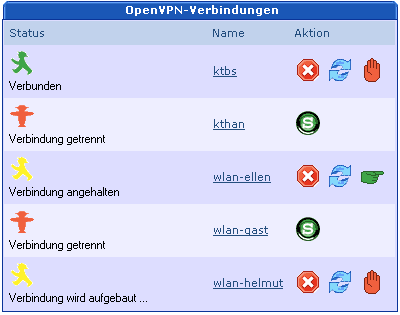
\includegraphics[width=400pt]{verbindungen}
    \caption{Verbindungsübersicht}
    \label{fig:guiact}
  \end{figure}

\begin{description}
\item [Status:] Der Status einer Verbindung wird mit Ampelmännchen
  symbolisiert. Ein rotes Männchen bedeutet, dass der OpenVPN-Prozess
  nicht läuft, ein gelbes, dass der Prozess zwar läuft aber (noch)
  keine Verbindung zur Gegenstelle aufgebaut werden konnte und ein
  grünes, dass die Verbindung mit der Gegenstelle \glqq{}steht\grqq{}.
  Genauere Informationen über den Status erhält man als Tooltip über
  dem Ampelmännchen. Das kann insbesondere bei \glqq{}gelbem\grqq{}
  Status aufschlussreich sein.

\item [Name:] In dieser Spalte steht der Name der OpenVPN-Verbindung
  wie er in der Konfiguration angegeben wurde. Ein Klick auf den Namen
  führt in eine Übersicht, in der genauere Informationen zu dieser
  Verbindung angezeigt werden. Dazu später mehr.

\item [Aktion:] Hier sind die zur Verfügung stehenden Aktionen als
  Buttons symbolisiert. Was sie jeweils bedeuten, erfährt man über
  Tooltips. Folgende Buttons gibt es:

  \begin{table}[!h]
    \begin{tabular}{lp{12cm}}
      Symbol                                         & Erläuterung \\
      \hline                                                            \\
      
\includegraphics[width=24pt]{start}            & Der OpenVPN-Prozess wird gestartet und es wird versucht eine Verbindung aufzubauen.        \\
      
\includegraphics[width=24pt]{stop}             & Der OpenVPN-Prozess wird beendet. \\
      
\includegraphics[width=24pt]{reload}           & Die Verbindung wird zurückgesetzt. \\
      
\includegraphics[width=24pt]{hold}             & Die Verbindung wird zurückgesetz und auf 'hold' geschaltet. Dann gehen keine Daten mehr über die Verbindung. \\
      
\includegraphics[width=24pt]{release}          & Die Verbindung wird wieder freigegeben. Daten können wieder über die Verbindung fließen.  \\
      \hline                                                            \\
    \end{tabular}
  \caption{Aktionen der OpenVPN-Webgui}
\end{table}
\end{description}

\subsubsection{OpenVPN - WebGUI - Detailansicht einer Verbindung}
  \begin{figure}[!h]
    \centering
    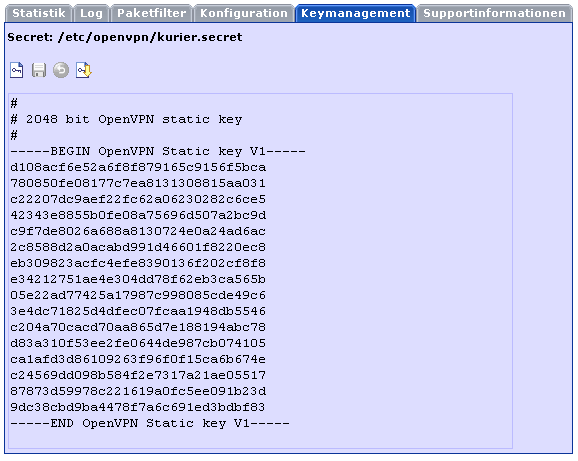
\includegraphics[width=400pt]{detail}
    \caption{Detailansicht einer Verbindung (Keymanagement)}
    \label{fig:guidetail}
  \end{figure}

\begin{description}
\item [Statistik:] Hier werden ein paar interessante Statistiken
    angezeigt.  Die Statistik kann nur angezeigt werden, wenn die
    Verbindung gestartet und nicht angehalten ist.

\item [Log:] Zeigt die letzten 20 Zeilen des Verbindungslogs.  Wenn
    Sie mehr Zeilen sehen möchten, können Sie auch deren Anzahl
    angeben und auf 'Anzeigen' klicken.  Wenn Sie als Anzahl 'all'
    einngeben, wird das gesamte Log angezeigt.  Dieser Reiter wird nur
    angezeigt, wenn die Verbindung gestartet ist.

\item [Debug-Log:] Zeigt die Ausgabe eines Startvorgangs.  Die
    OpenVPN-Verbindung wird gestartet und die Ausgaben dabei
    angezeigt.  Das ist dann nützlich, wenn die Verbindung über den
    Start Button nicht starten will und man dadurch kein normales Log
    zu sehen bekommt.  Dieser Reiter wird nur angezeigt, wenn die
    Verbindung nicht gestartet ist.

\item [Paketfilter:] Zeigt die Paketfilterkonfiguration an, die für
    diese Verbindung gültig ist. Der Paketfilter ist nur konfiguriert,
    wenn die Verbindung gestartet und als Tunnel eingerichtet ist.

\item [Bridge:] Zeigt die Konfiguration der Bridges auf dem Router
    an. Dieser Punkt nur angezeigt, wenn die Verbindung als Bridge
    eingerichtet ist.

\item [Konfiguration:] Über diesen Punkt kann die beim Booten
    generierte Konfiguration der Verbindung angeschaut werden.

\item [Keymanagement:] Über diesen Punkt kann für diese Verbindung ein
    Schlüssel erzeugt und auch heruntergeladen werden. (siehe
    Abbildung \ref{fig:guidetail}) Ist kein Schlüssel vorhanden (beim
    ersten Start) wird automatisch einer generiert und angezeigt. Er
    kann über das Download-Symbol direkt heruntergeladen, oder mit
    copy/paste in eine Textdatei übertragen werden. Um einen neu
    generierten Schlüssel auf dem Router zu speichern, ist auf das
    Disketten-Symbol zu klicken. Ein solcher Speichervorgang kann mit
    einem Klick auf das Wiederherstellen Symbol rückgängig gemacht
    werden.

\item [Supportinformationen:] Hier werden alle Dinge angezeigt, die
    bei Problemen relevant sein könnten.  Sie können diese
    Informationen dann beispielsweise auf Anfrage per copy\&paste in
    einen Artikel der Newsgroup übertragen.

\end{description}


\subsection{OpenVPN - Zusammenarbeit unterschiedlicher OpenVPN Versionen}

Bei der Zusammenarbeit unterschiedlicher OpenVPN Versionen muss darauf
geachtet werden, dass diese unterschiedliche Standardwerte für die
Parameter einer Verbindung benutzen. Das betrifft insbesondere die
MTU, Fragment und MSSFIX Einstellungen. Wenn die entsprechenden Werte
nicht \glqq{}zusammenpassen\grqq{}, ist ein Verbindungsaufbau nicht
möglich oder die Verbindung funktioniert zwar mit einem Pingbefehl,
bricht aber beispielsweise bei der Benutzung von ssh
zusammen. Typische Fehlermeldungen in einem solchen Fall sind z. B.:

\begin{example}
\begin{verbatim}
FRAG_IN error flags=0xfa2a187b: FRAG_TEST not implemented
FRAG_IN error flags=0xfa287f34: spurrious FRAG_WHOLE flags
\end{verbatim}
\end{example}

Die entscheidenden Parameter für das Zustandekommen einer Verbindung
sind folgende Einstellungen:

\begin{description}

\item [OPENVPN\_x\_TUN\_MTU] Der MTU Wert des TUN Geräte war bei
  OpenVPN 1.x auf 1300 eingestellt. Ab OpenVPN 2.0 wird 1500 als
  Standardwert angenommen.

\item [OPENVPN\_x\_LINK\_MTU] Die Bytegröße der Verbindung der beiden
  OpenVPN Daemonen. Dieser Standardwert ist abhängig von der
  verwendeten OpenVPN Version und des Betriebssystems.

\item [OPENVPN\_x\_FRAGMENT] Datenpakete (egal ob UDP oder TCP), deren
  Größe über der Fragmentgrenze liegt, werden auf Datenpakete
  aufgeteilt, die nicht größer sind als die unter \var{OPENVPN\_x\_FRAGMENT}
  angegeben Bytegröße.

\item [OPENVPN\_x\_MSSFIX] Damit TCP Verbindungen, die über das VPN
  Daten austauschen, nach Möglichkeit die Datenpakete nicht
  fragmentieren müssen, kann hier eine gewünschte maximale Größe der
  TCP Datenpakete vorgegeben werden. An diese Vorgabe halten sich dann
  aktuelle Betriebssysteme und ein aufwendiges fragmentieren der
  Datenpakete ist nicht notwendig.

\end{description}

Die unterschiedlichen OpenVPN Versionen benutzen folgende Werte als
Standardwerte. Diese Werte müssen Sie beachten, wenn Sie mit OpenVPN
Versionen Kontakt aufnehmen wollen, die nicht auf einem fli4l-Router
laufen. Die Standardwerte auf dem fli4l-Router sind in der zweiten
Tabelle aufgeführt.

\begin{table}[htbp]
  \begin{scriptsize}
    \begin{tabular}{lll}
      OpenVPN Version/Option        & 1.xx                & 2.00        \\
      \hline                                                    \\
      OPENVPN\_x\_TUN\_MTU          & 1300                & 1500        \\
      OPENVPN\_x\_TUN\_MTU\_EXTRA   & unbekannt           & 32          \\
      OPENVPN\_x\_FRAGMENT          & unbekannt           & nicht konfiguriert  \\
      OPENVPN\_x\_MSSFIX            & nicht konfiguriert  & 1450        \\
    \end{tabular}
  \end{scriptsize}
  \caption{Unterschiedliche MTU Parameter der unterschiedlichen OpenVPN Versionen.}
\end{table}

\begin{table}[htbp]
  \begin{scriptsize}
    \begin{tabular}{lll}
      fli4l Version/Option          & bis einschließlich 2.1.8  & ab 2.1.9  \\
      \hline                                                    \\
      OPENVPN\_x\_TUN\_MTU          & 1300                & 1500        \\
      OPENVPN\_x\_TUN\_MTU\_EXTRA   & 64                  & 32          \\
      OPENVPN\_x\_FRAGMENT          & nicht konfiguriert  & 1300        \\
      OPENVPN\_x\_MSSFIX            & nicht konfiguriert  & 1300        \\
    \end{tabular}
  \end{scriptsize}
  \caption{Unterschiedliche MTU Parameter der fli4l-Router Versionen.}
\end{table}

Aufgrund dieser unterschiedlichen Einstellungen, sollten Sie die für
Ihr Netzwerk passenden Standardwerte ermitteln und diese dann explizit
in die config/openvpn.txt schreiben. Folgende Werte sind in den
meisten Fällen gute Startwerte für die ersten Tests.

\begin{example}
\begin{verbatim}
OPENVPN_DEFAULT_TUN_MTU='1500'
OPENVPN_DEFAULT_MSSFIX='1300'
OPENVPN_DEFAULT_FRAGMENT='1300'
\end{verbatim}
\end{example}

Leider gibt es für fli4l Versionen vor 2.1.9 keine Möglichkeit den
\glqq{}tun-mtu\grqq{} Parameter direkt zu setzen. Allerdings läßt sich
dieser Parameter indirekt über den \var{OPENVPN\_x\_LINK\_MTU}
beeinflussen. Der tun-mtu Wert ist ca. 45 Bytes kleiner als der bei
\var{OPENVPN\_x\_LINK\_MTU} angegebene Wert. Um den genauen Wert zu
ermitteln, hilft nur ausprobieren.

\subsection{OpenVPN - Beispiele}

Einige Beispiele verdeutlichen die Konfiguration des OpenVPN Paketes.

\subsubsection{Beispiel - Zwei Netze mit fli4l-Routern verbinden}

Im ersten Beispiel werden zwei fli4l-Router miteinander verbunden.
Die Netzwerke hinter den fli4l-Routern sollen dabei Zugriff auf das
jeweils andere Netzwerk erhalten. In diesem Beispiel wollen Peter und
Maria ihre Netzwerke über ihre fli4l-Router miteinander verbinden.
Peter benutzt als privates Netz 192.168.145.0/24 und als DynDNS
Adresse 'peter.eisfair.net'. Bei Maria sieht es ähnlich aus, nur
benutzt sie das Netzwerk 10.23.17.0/24 und als DynDNS Adresse
'maria.eisfair.net'. Das sich beide unbegrenzt vertrauen, erlauben sie
sich gegenseitig den kompletten Zugriff auf ihre jeweiligen Netze.

\begin{table}[htbp]
  \begin{scriptsize}
    \begin{tabular}{lll}
      OpenVPN Option                & Peter              & Maria               \\
      \hline \\
      OPENVPN\_1\_NAME=             & 'maria'            & 'peter'             \\
      OPENVPN\_1\_REMOTE\_HOST=     & 'maria.eisfair.net' & 'peter.eisfair.net' \\
      OPENVPN\_1\_REMOTE\_PORT=     & '10000'            & '10001'             \\
      OPENVPN\_1\_LOCAL\_PORT=      & '10001'            & '10000'             \\
      OPENVPN\_1\_SECRET=           & 'pema.secret'      & 'pema.secret'       \\
      OPENVPN\_1\_TYPE=             & 'tunnel'           & 'tunnel'            \\
      OPENVPN\_1\_REMOTE\_VPN\_IP=  & '192.168.200.202'  & '192.168.200.193'   \\
      OPENVPN\_1\_LOCAL\_VPN\_IP=   & '192.168.200.193'  & '192.168.200.202'   \\
      OPENVPN\_1\_ROUTE\_N=         & '1'                & '1'                 \\
      OPENVPN\_1\_ROUTE\_1=         & '10.23.17.0/24'    & '192.168.145.0/24'  \\
      OPENVPN\_1\_PF\_INPUT\_N=   & '1'                & '1'                 \\
      OPENVPN\_1\_PF\_INPUT\_1=   & 'ACCEPT'           & 'ACCEPT'            \\
      OPENVPN\_1\_PF\_FORWARD\_N= & '1'                & '1'                 \\
      OPENVPN\_1\_PF\_FORWARD\_1= & 'ACCEPT'  & 'ACCEPT' \\
    \end{tabular}
  \end{scriptsize}
  \caption{OpenVPN Konfiguration mit 2 fli4l-Routern}
\end{table}

\subsubsection{Beispiel - Zwei Netze mit einer Bridge verbinden}

Im nächsten Beispiel wird eine Bridge über eine Funkverbindung
aufgebaut. Bei einer Bridge kann der Paketfilter nicht sinnvoll
konfiguriert werden, da dort nur Ethernetframes weitergeleitet werden,
aber nicht unbedingt IP-Pakete. Bitte immer daran denken, dass bei
einer Bridgekonfiguration ein gemeinsames Netz benutzt werden
muss. Und es dürfen keine IP-Adressen doppelt vergeben werden.

\begin{table}[htbp]
  \begin{scriptsize}
    \begin{tabular}{lll}
      OpenVPN Option           & Peter           & Maria           \\
      \hline \\
      OPENVPN\_2\_NAME         & 'bridge'        & 'bridge'          \\
      OPENVPN\_2\_REMOTE\_HOST & '10.1.0.1'      & '10.2.0.1'      \\
      OPENVPN\_2\_REMOTE\_PORT & '10005'         & '10006'         \\
      OPENVPN\_2\_LOCAL\_HOST  & '10.2.0.1'      & '10.1.0.1'      \\
      OPENVPN\_2\_LOCAL\_PORT  & '10006'         & '10005'         \\
      OPENVPN\_2\_FLOAT        & 'no'            & 'no'            \\
      OPENVPN\_2\_RESTART      & 'never'         & 'never'         \\
      OPENVPN\_2\_SECRET       & 'bridge.secret' & 'bridge.secret' \\
      OPENVPN\_2\_TYPE         & 'bridge'        & 'bridge'        \\
      OPENVPN\_2\_BRIDGE       & 'pema-br'       & 'pema-br'       \\
    \end{tabular}
  \end{scriptsize}
  \caption{OpenVPN Konfiguration mit 2 fli4l-Routern deren Netzwerk über eine Funkverbindung gebridgt wird.}
\end{table}

Zusätzlich zu den Angaben für OpenVPN muss natürlich noch eine Bridge
in advanced\_networking konfiguriert werden und die base.txt so
angepaßt werden, dass dort die Bridge und nicht eth0 als
Netzwerkdevice für das interne Netzwerk benutzt wird. Hier nochmal die
relevanten Auszüge aus der Konfiguration von advanced\_networking und
base.

\begin{table}[htbp]
  \begin{scriptsize}
    \begin{tabular}{lll}
      advanced\_networking Option  & Peter           & Maria       \\
      \hline \\
      OPT\_BRIDGE\_DEV             & 'yes'           & 'yes'       \\
      BRIDGE\_DEV\_BOOTDELAY       & 'no'            & 'no'        \\
      BRIDGE\_DEV\_N               & '1'             & '1'         \\
      BRIDGE\_DEV\_1\_NAME         & 'pema-br'       & 'pema-br'   \\
      BRIDGE\_DEV\_1\_DEVNAME      & 'br0'           & 'br0'       \\
      BRIDGE\_DEV\_1\_DEV\_N       & '1'             & '1'         \\
      BRIDGE\_DEV\_1\_DEV\_1\_DEV  & 'eth0'          & 'eth0'      \\
    \end{tabular}
  \end{scriptsize}
  \caption{OpenVPN Konfiguration mit 2 fli4l-Routern deren Netzwerk über eine Funkverbindung gebridgt wird. Die Konfiguration der Bridge in advanced\_networking.}
\end{table}

\begin{table}[htbp]
  \begin{scriptsize}
    \begin{tabular}{lll}
      base Option  & Peter           & Maria       \\
      \hline \\
      IP\_NET\_N            & '1'                   & '1'                    \\
      IP\_NET\_1            & '192.168.193.254/24'  & '192.168.193.1/24'     \\
      IP\_NET\_1\_DEV       & 'br0'                 & 'br0'                  \\
    \end{tabular}
  \end{scriptsize}
  \caption{OpenVPN Konfiguration mit 2 fli4l-Routern deren Netzwerk über eine Funkverbindung gebridgt wird. Die Konfiguration der Bridge in der Basiskonfiguration (base.txt).}
\end{table}

\subsubsection{Beispiel - Zugriff für einen Roadwarrior konfigurieren}

\marklabel{roadwarrior}Bei diesem Beispiel (Roadwarrior) wird über ein
Notebook mit Windows XP und einem GPRS Zugang der Zugang zu dem LAN
hinter dem fli4l-Router ermöglicht.  Dazu wird auf dem Windows XP
Notebook OpenVPN installiert und die entsprechende *.ovpn Datei
angepaßt.  Leider ist der tun/tap Treiber unter Windows nicht ganz so
flexibel wie sein Unix Gegenstück. Daher müssen die
Point-to-Pointadressen für die VPN IP-Adressen in einem
255.255.255.252 (oder /30) Netz liegen. Wenn der Roadwarrior nur auf
Dienste im LAN hinter und auf dem fli4l-Router zugreifen soll und
nicht selber angesprochen werden muss, ist die Angabe einer Route auf
der fli4l Seite nicht notwendig. Der Roadwarrior kann bei Bedarf über
seine virtuelle IP-Adresse (\var{OPENVPN\_3\_REMOTE\_VPN\_IP})
angesprochen werden. Wenn der Roadwarrior über eine feste IP-Adresse
verfügt, könnte man auch alternativ eine Hostroute eintragen. Wenn der
Roadwarrior z.B. die feste IP-Adresse 192.168.33.33 hat, könnte man
folgendes noch in die fli4l openvpn.txt Konfigurationsdatei einfügen:

\begin{example}
\begin{verbatim}
OPENVPN_3_ROUTE_N='1'
OPENVPN_3_ROUTE_1='192.168.33.33/32'
\end{verbatim}
\end{example}

Mit der Paketfilterkonfiguration, die hier im Beispiel gezeigt wird
erlauben wir wieder die komplette Kommunikation in beide
Richtungen. Nur auf den fli4l-Router direkt kann der Roadwarrior nicht
zugreifen. Das wäre z.B. notwendig, wenn der Roadwarrior den DNS
Server auf dem fli4l-Router benutzen soll.

\begin{example}
\begin{verbatim}
OPENVPN_3_PF_FORWARD_N='1'
OPENVPN_3_PF_FORWARD_1='ACCEPT'
\end{verbatim}
\end{example}

Soll der Zugriff vom Roadwarrior auf den internen DNS Server auf dem
fli4l-Router erlaubt werden, muss noch folgendes zur fli4l
Konfiguration dazugeschrieben werden:

\begin{example}
\begin{verbatim}
OPENVPN_3_PF_INPUT_N='1'
OPENVPN_3_PF_INPUT_1='if:VPNDEV:any tmpl:dns ACCEPT'
\end{verbatim}
\end{example}

\begin{table}[htbp]
  \begin{scriptsize}
    \begin{tabular}{ll}
      OpenVPN Option fli4l-Router                   & roadwarrior           \\
      \hline \\
      OPENVPN\_3\_NAME='roadwarrior'                & remote peter.eisfair.net \\
      OPENVPN\_3\_LOCAL\_PORT='10011'               & rport 10011 \\
      OPENVPN\_3\_SECRET='roadwarrior.secret'       & secret roadwarrior.secret \\
      OPENVPN\_3\_TYPE='tunnel'                     & dev tun \\
      OPENVPN\_3\_REMOTE\_VPN\_IP='192.168.200.238' & ~ \\
      OPENVPN\_3\_LOCAL\_VPN\_IP='192.168.200.237'  & ifconfig 192.168.200.238 192.168.200.237 \\
      OPENVPN\_3\_ROUTE\_N='0'                      & ~ \\
      OPENVPN\_3\_PF\_FORWARD\_N='1'              & ~ \\
      OPENVPN\_3\_PF\_FORWARD\_1='ACCEPT' & ~ \\
      ~                                             & route 192.168.145.0 255.255.255.0 \\
      ~                                             & comp-lzo \\
      ~                                             & persist-tun \\
      ~                                             & persist-key \\
      ~                                             & ping-timer-rem \\
      ~                                             & ping-restart 60 \\
      ~                                             & proto udp4 \\
      ~                                             & tun-mtu 1500 \\
      ~                                             & fragment 1300 \\
      ~                                             & mssfix \\
    \end{tabular}
  \end{scriptsize}
  \caption{OpenVPN Konfiguration mit einem Windowsrechner über GPRS.}
\end{table}

\subsubsection{Beispiel - WLAN Verbindung absichern}

In diesem Beispiel wird eine WLAN Verbindung mit Hilfe von OpenVPN
abgesichert. Es wird davon ausgegangen, dass im fli4l-Router sowohl
eine LAN als auch eine WLAN Karte verwendet wird, oder ein Accesspoint
an einer zusätzlichen Netzwerkkarte im fli4l angeschlossen ist. Ziel
soll es sein, dass ein WLAN Client ohne VPN-Verbindung lediglich
Zugriff auf den VPN Port des fli4l-Routers hat. Erst nach dem
erfolgreichen Verbinden mit OpenVPN, soll uneingeschränkter Austausch
mit dem Kabelgebundenen LAN möglich sein.  Es müssen dafür auch
Änderungen am DNSMASQ DHCP Server durchgeführt werden.  Außerdem wird
das advanced\_networking Paket benötigt.  Einstellungen in base.txt:
\var{IP\_NET\_1} ist dabei das kabelgebundene LAN und \var{IP\_NET\_2}
das WLAN.
\begin{example}
\begin{verbatim}
IP_NET_N='2'
IP_NET_1='192.168.3.254/24'
IP_NET_1_DEV='br0'
IP_NET_2='192.168.4.254/24'
IP_NET_2_DEV='eth2'
\end{verbatim}
\end{example}

Die DHCP-Range ist nach Belieben einzustellen.  Für \var{IP\_NET\_2}
sind aber unbedingt folgende Einstellungen hinzuzufügen:

\begin{example}
\begin{verbatim}
DHCP_RANGE_2_DNS_SERVER1='none'  
DHCP_RANGE_2_NTP_SERVER='none'  
DHCP_RANGE_2_GATEWAY='none' 
\end{verbatim}
\end{example}

Einstellung in advanced\_networking.txt:
\begin{example}
\begin{verbatim}
OPT_BRIDGE_DEV='yes'
BRIDGE_DEV_BOOTDELAY='yes'
BRIDGE_DEV_N='1'
BRIDGE_DEV_1_NAME='br'
BRIDGE_DEV_1_DEVNAME='br0'
BRIDGE_DEV_1_DEV_N='1'
BRIDGE_DEV_1_DEV_1_DEV='eth0'
\end{verbatim}
\end{example}

\begin{table}[htbp]
  \begin{scriptsize}
    \begin{tabular}{ll}
      OpenVPN Option Router                         & WLAN-Client         \\
      \hline \\
      OPENVPN\_4\_NAME='wlan1'                      & ~ \\
      OPENVPN\_4\_LOCAL\_HOST='192.168.4.254'       & remote 192.168.4.254\\
      OPENVPN\_4\_LOCAL\_PORT='20001'               & rport 20001 \\
      OPENVPN\_4\_SECRET='wlan1.secret'             & secret wlan1.secret \\
      OPENVPN\_4\_TYPE='bridge'                     & dev tap\\
      OPENVPN\_4\_BRIDGE='br'                       & ~\\
      OPENVPN\_4\_RESTART='never'                   & ~\\
      OPENVPN\_4\_MUTE\_REPLAY\_WARNINGS='yes'      & ~\\
      ~                                             & comp-lzo \\
      ~                                             & persist-tun \\
      ~                                             & persist-key \\
      ~                                             & ping-timer-rem \\
      ~                                             & ping-restart 60 \\
      ~                                             & proto udp4 \\
      ~                                             & tun-mtu 1500 \\
      ~                                             & fragment 1300 \\
      ~                                             & mssfix \\
    \end{tabular}
  \end{scriptsize}
  \caption{OpenVPN Absicherung eines WLAN.}
\end{table}

\subsection{Weiterführende Links zum Thema OpenVPN}

Abschliessend noch einige Links, die sich mit der Konfiguration von
OpenVPN beschäftigen:

\noindent \altlink{http://openvpn.net} \\
\altlink{http://de.wikipedia.org/wiki/OpenVPN} \\
\altlink{http://openvpn.se/} \\
% \altlink{http://www.vpnforum.de/} \\
\altlink{http://arnowelzel.de/wiki/de/fli4l/openvpn} \\
\altlink{http://wiki.freifunk.net/OpenVPN} \\
\altlink{http://w3.linux-magazine.com/issue/24/Charly.pdf} \\
\altlink{http://w3.linux-magazine.com/issue/25/WirelessLAN_Intro.pdf} \\
\altlink{http://w3.linux-magazine.com/issue/25/OpenVPN.pdf} \\
% \altlink{http://www.0dx.de/linux/linuxmag/1994_2009/2002/08/sysadauf/sysadauf.html} \\
% \altlink{http://bilbo.naumann-net.org/~ms/aklininst/folien/01/openvpn.pdf} \\
% \altlink{http://lists.spline.inf.fu-berlin.de/pipermail/fli4l_dev/2005-May/016101.html} \\
